\documentclass[11pt,a4paper]{article}
\usepackage[utf8]{inputenc}
\usepackage{amsmath}
\usepackage{amsfonts}
\usepackage{amssymb}
\usepackage{xcolor}
\usepackage{array,booktabs}
\usepackage[none]{hyphenat}
\usepackage{geometry}
\usepackage{graphicx}
\geometry{margin=2.5cm}
\usepackage{float}
\usepackage{multirow}
\usepackage{amsthm}
\usepackage{hyperref}
\theoremstyle{plain}
\usepackage{graphicx}
\usepackage{caption}
\usepackage{subcaption}
\newtheorem{thm}{Theorem}[section] % reset theorem numbering for each chapter

\theoremstyle{definition}
\newtheorem{defn}[thm]{Definition} % definition numbers are dependent on theorem numbers
\newtheorem{exmp}[thm]{Example} % same for example numbers
%\usepackage{cmbright}
\usepackage{fancyhdr}
\pagestyle{fancy}
\fancyhf{}
\rhead{Biharmonic Test}
\lhead{\leftmark}
\rfoot{\thepage}
\author{}
\title{}
\begin{document}
In this tests we consider:
\begin{itemize}
\item $\psi(x)=x^3$
\item $\psi_\text l=0$
\item $\psi_\text r=1$
\item $\psi_\text{ll}=0$
\item $\psi_\text{rr}=3$
\item $g(x)=0$
\end{itemize}
\begin{table}[H]
\caption{(normal)}
\setlength{\tabcolsep}{5pt}
\centering
\begin{tabular}{@{}l c c c@{}}
\toprule
 &  & \multicolumn{2}{c}{PRO1}\\
\midrule
 & $I$ & E$_{0,I}(E_{\infty})$ & E$_{0,I}(O_{\infty})$\\
\midrule
\multirow{6}{*}{$\mathbb{P}_{3}$}
 & 20 & 3.04E$-$14 & ---\\
 & 40 & 1.16E$-$13 & $\uparrow$\\
 & 80 & 1.53E$-$13 & $\uparrow$\\
 & 160 & 2.67E$-$12 & $\uparrow$\\
 & 320 & 2.41E$-$11 & $\uparrow$\\
 & 640 & 2.59E$-$10 & $\uparrow$\\
\midrule
\multirow{6}{*}{$\mathbb{P}_{5}$}
 & 20 & 2.00E$-$14 & ---\\
 & 40 & 2.59E$-$13 & $\uparrow$\\
 & 80 & 1.00E$-$12 & $\uparrow$\\
 & 160 & 4.45E$-$12 & $\uparrow$\\
 & 320 & 1.28E$-$10 & $\uparrow$\\
 & 640 & 3.37E$-$10 & $\uparrow$\\
\bottomrule
\end{tabular}
\label{Table:PRO:test_01_01_test47_pro1}
\end{table}

\begin{table}[H]
\caption{(consistency)}
\setlength{\tabcolsep}{5pt}
\centering
\begin{tabular}{@{}l c c c@{}}
\toprule
 &  & \multicolumn{2}{c}{PRO1}\\
\midrule
 & $I$ & E$_{0,I}(E_{\infty})$ & E$_{0,I}(O_{\infty})$\\
\midrule
\multirow{6}{*}{$\mathbb{P}_{3}$}
 & 20 & 3.24E$-$11 & ---\\
 & 40 & 3.27E$-$10 & $\uparrow$\\
 & 80 & 5.78E$-$09 & $\uparrow$\\
 & 160 & 1.07E$-$07 & $\uparrow$\\
 & 320 & 1.96E$-$06 & $\uparrow$\\
 & 640 & 6.07E$-$05 & $\uparrow$\\
\midrule
\multirow{6}{*}{$\mathbb{P}_{5}$}
 & 20 & 1.08E$-$09 & ---\\
 & 40 & 6.19E$-$10 & 0.81\\
 & 80 & 5.19E$-$08 & $\uparrow$\\
 & 160 & 8.52E$-$07 & $\uparrow$\\
 & 320 & 6.58E$-$06 & $\uparrow$\\
 & 640 & 2.31E$-$04 & $\uparrow$\\
\bottomrule
\end{tabular}
\label{Table:PRO:test_01_01_test47_pro1}
\end{table}


\begin{figure}[H]
\begin{subfigure}[b]{0.48\textwidth}
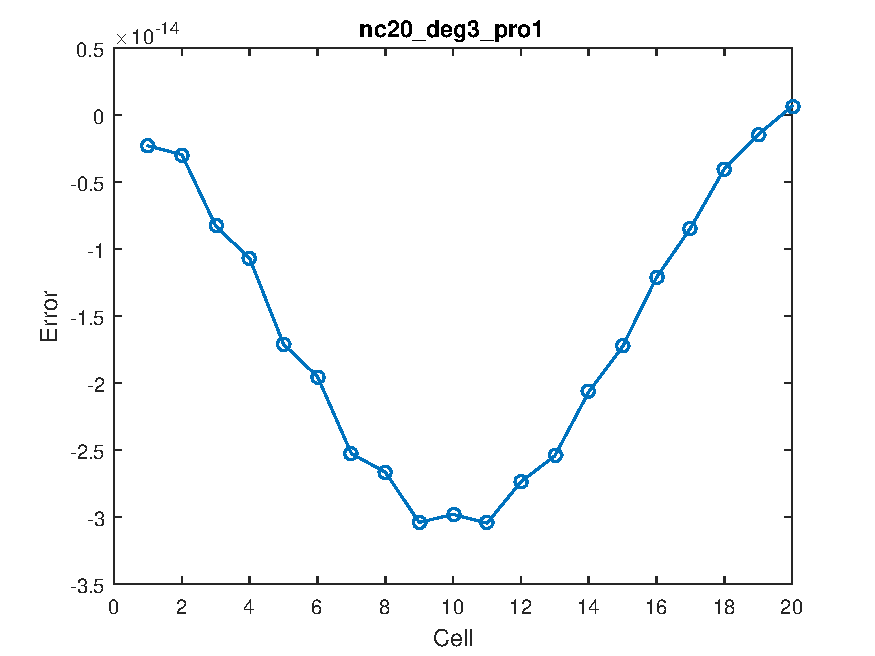
\includegraphics[width=\linewidth]{../../tests_01_01/test_01_01_test47_pro1/output/plots/nc20_deg3_wei111_pro1.pdf}
\end{subfigure}\hspace*{\fill}
\begin{subfigure}[b]{0.48\textwidth}
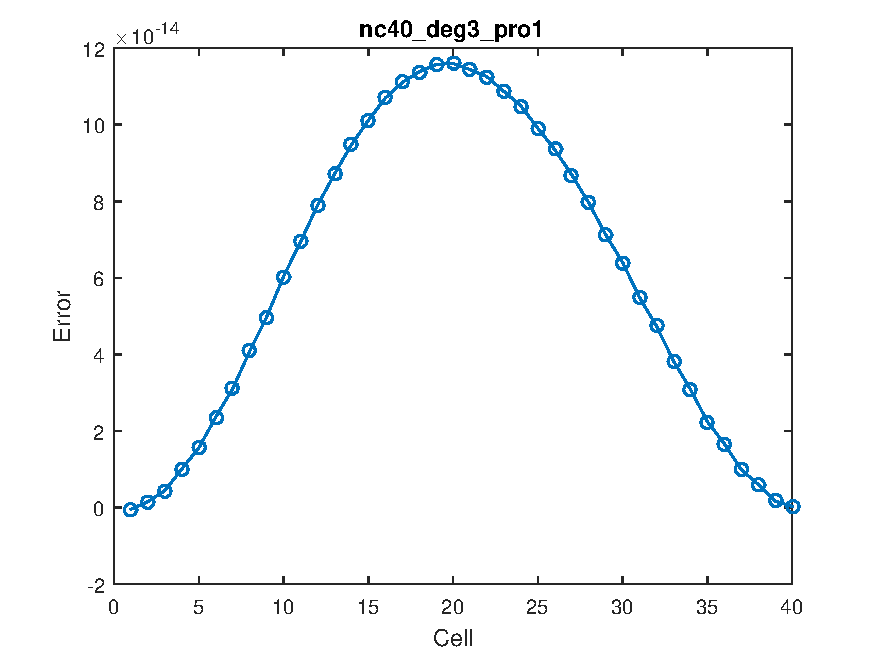
\includegraphics[width=\linewidth]{../../tests_01_01/test_01_01_test47_pro1/output/plots/nc40_deg3_wei111_pro1.pdf}
\end{subfigure}

\medskip
\begin{subfigure}[b]{0.48\textwidth}
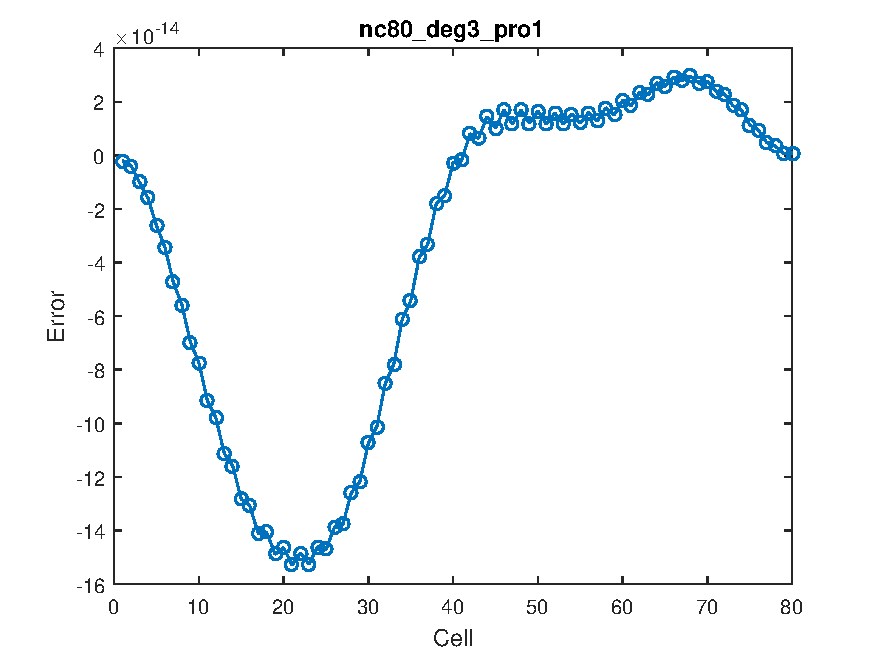
\includegraphics[width=\linewidth]{../../tests_01_01/test_01_01_test47_pro1/output/plots/nc80_deg3_wei111_pro1.pdf}
\end{subfigure}\hspace*{\fill}
\begin{subfigure}[b]{0.48\textwidth}
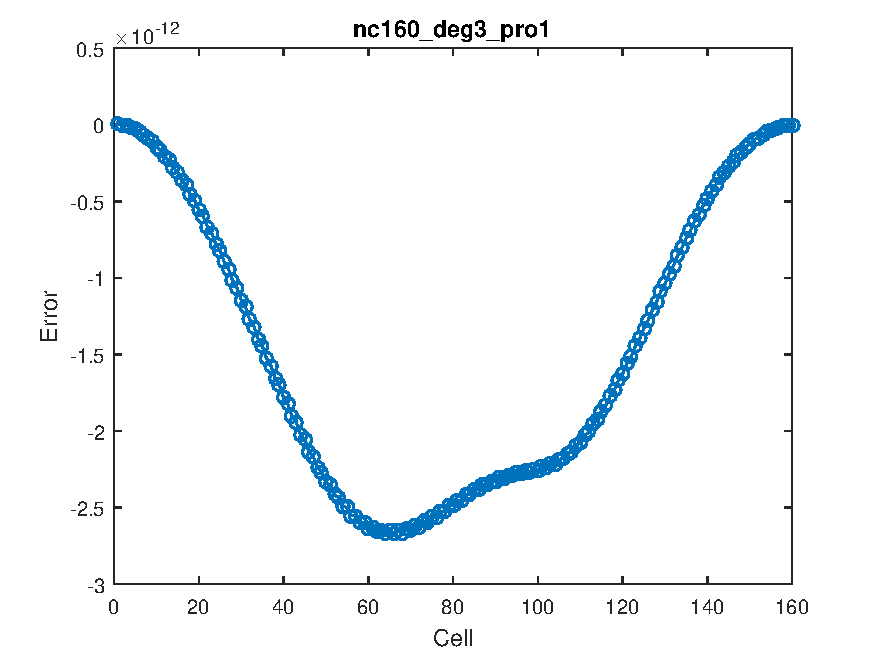
\includegraphics[width=\linewidth]{../../tests_01_01/test_01_01_test47_pro1/output/plots/nc160_deg3_wei111_pro1.pdf}
\end{subfigure}

\medskip
\begin{subfigure}[b]{0.48\textwidth}
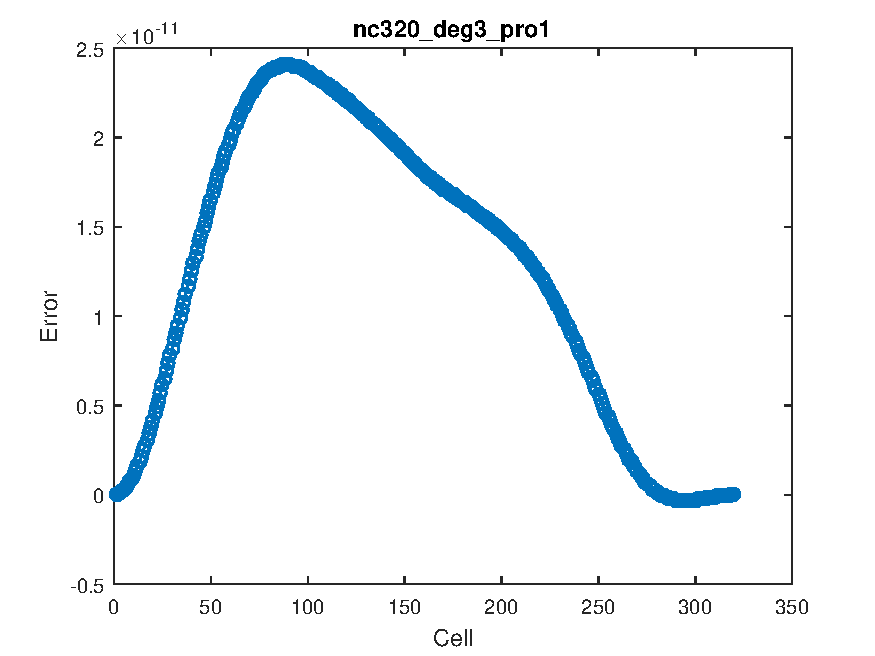
\includegraphics[width=\linewidth]{../../tests_01_01/test_01_01_test47_pro1/output/plots/nc320_deg3_wei111_pro1.pdf}
\end{subfigure}\hspace*{\fill}
\begin{subfigure}[b]{0.48\textwidth}
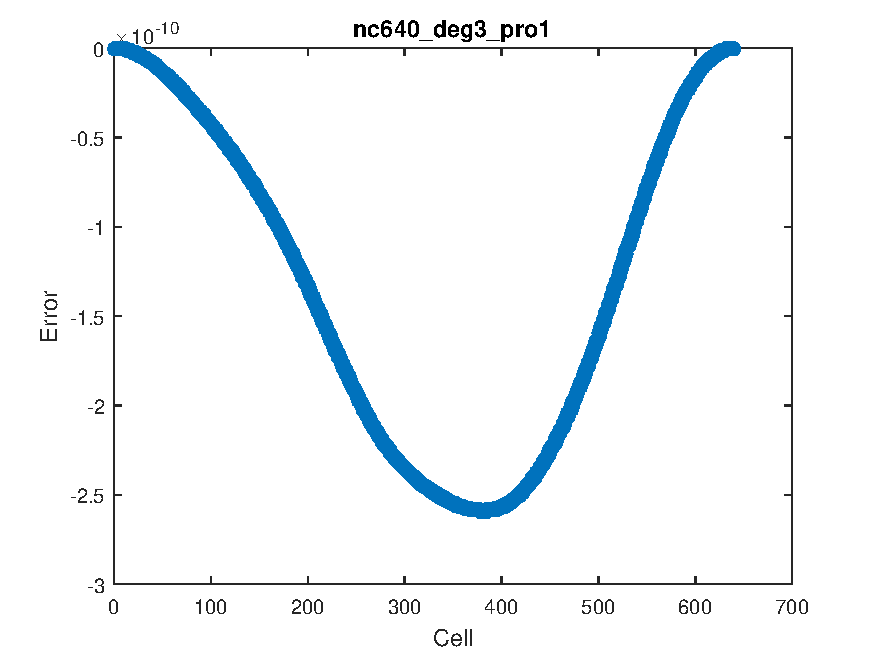
\includegraphics[width=\linewidth]{../../tests_01_01/test_01_01_test47_pro1/output/plots/nc640_deg3_wei111_pro1.pdf}
\end{subfigure}

\caption{$\omega=1|1,1$, d=3}
\end{figure}
%%%% 2
\begin{figure}[H]
\begin{subfigure}[b]{0.48\textwidth}
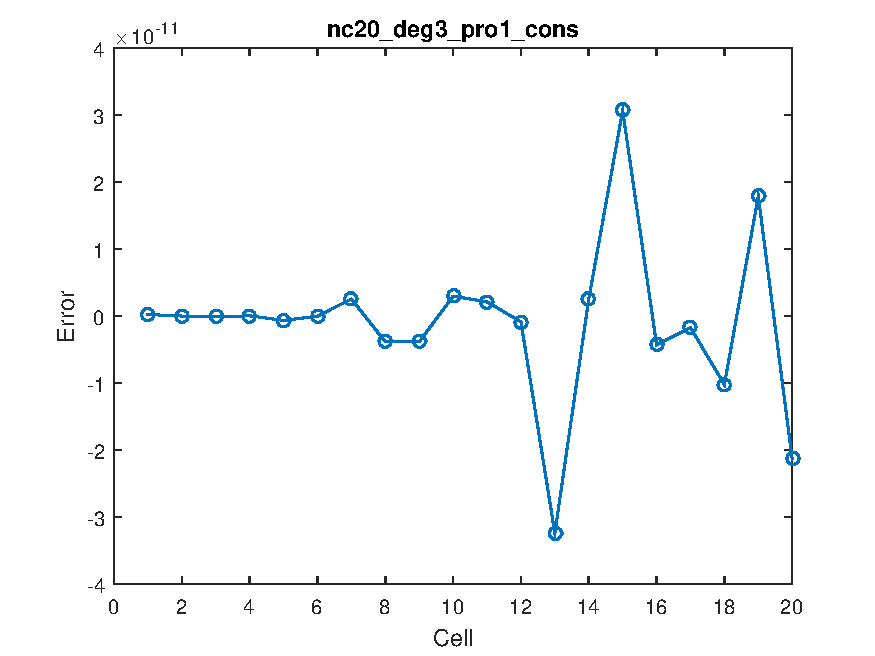
\includegraphics[width=\linewidth]{../../tests_01_01/test_01_01_test47_pro1_cons/output/plots/nc20_deg3_wei111_pro1_cons.pdf}
\end{subfigure}\hspace*{\fill}
\begin{subfigure}[b]{0.48\textwidth}
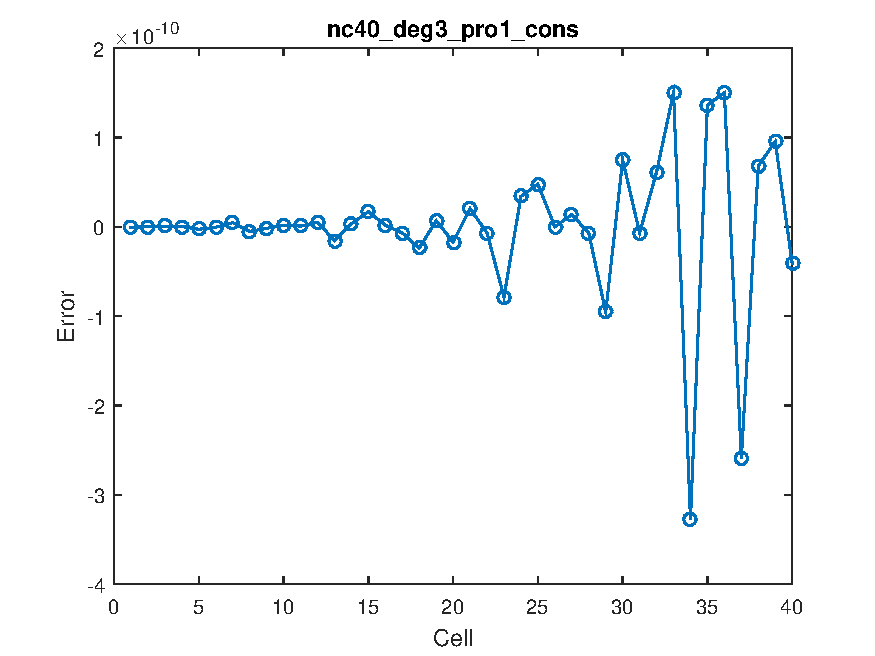
\includegraphics[width=\linewidth]{../../tests_01_01/test_01_01_test47_pro1_cons/output/plots/nc40_deg3_wei111_pro1_cons.pdf}
\end{subfigure}

\medskip
\begin{subfigure}[b]{0.48\textwidth}
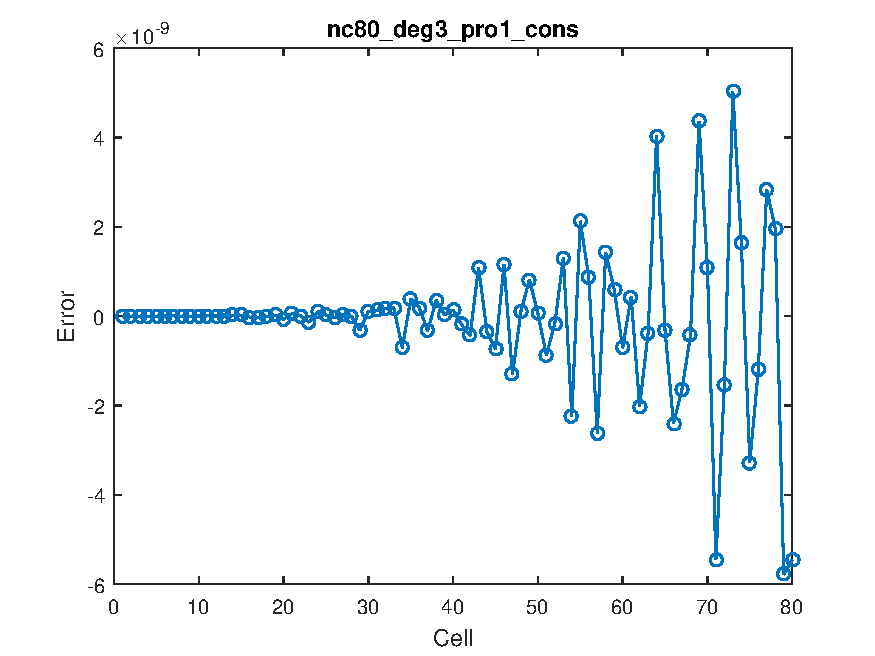
\includegraphics[width=\linewidth]{../../tests_01_01/test_01_01_test47_pro1_cons/output/plots/nc80_deg3_wei111_pro1_cons.pdf}
\end{subfigure}\hspace*{\fill}
\begin{subfigure}[b]{0.48\textwidth}
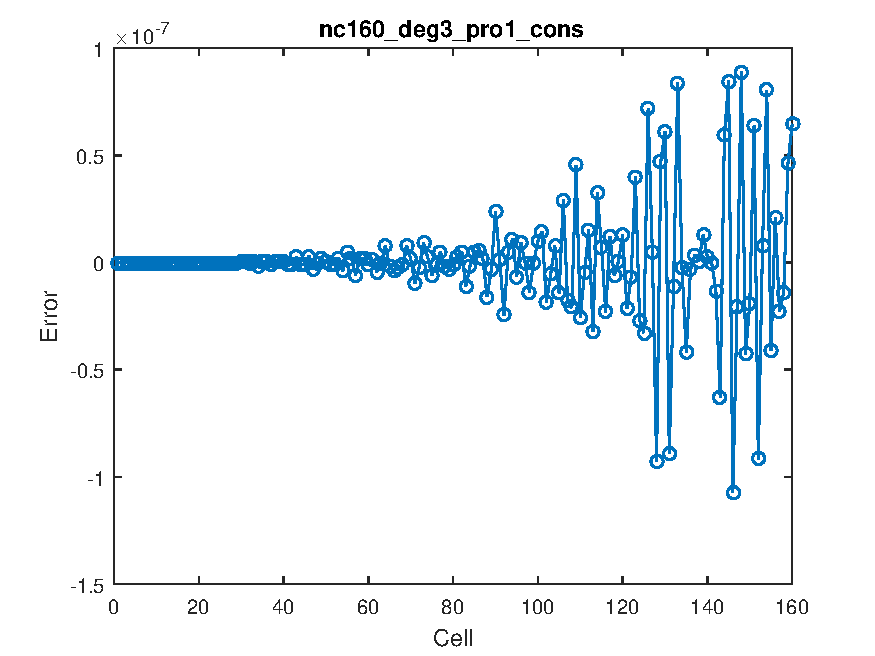
\includegraphics[width=\linewidth]{../../tests_01_01/test_01_01_test47_pro1_cons/output/plots/nc160_deg3_wei111_pro1_cons.pdf}
\end{subfigure}

\medskip
\begin{subfigure}[b]{0.48\textwidth}
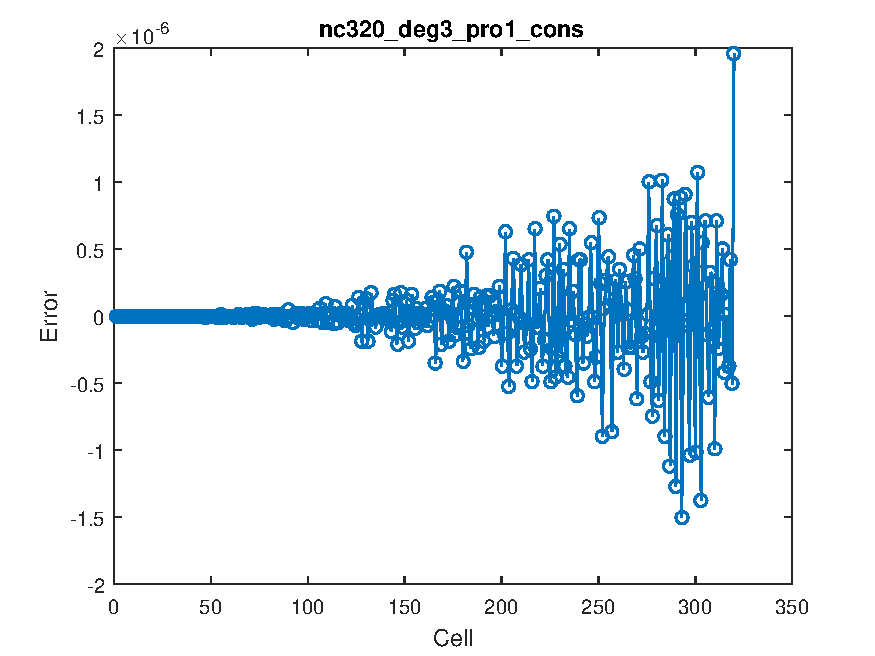
\includegraphics[width=\linewidth]{../../tests_01_01/test_01_01_test47_pro1_cons/output/plots/nc320_deg3_wei111_pro1_cons.pdf}
\end{subfigure}\hspace*{\fill}
\begin{subfigure}[b]{0.48\textwidth}
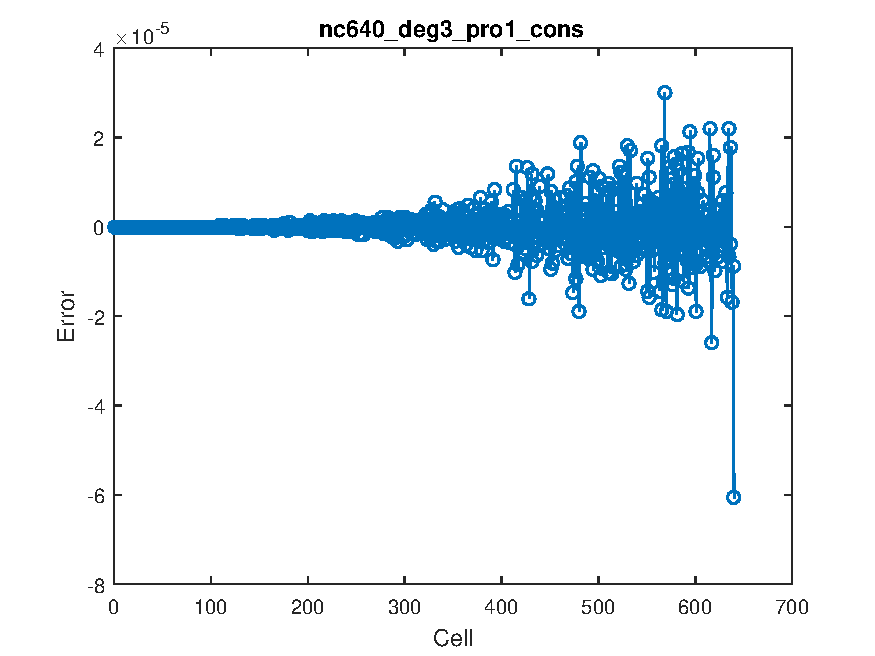
\includegraphics[width=\linewidth]{../../tests_01_01/test_01_01_test47_pro1_cons/output/plots/nc640_deg3_wei111_pro1_cons.pdf}
\end{subfigure}

\caption{$\omega=1|1,1$, d=3 (consistency)}
\end{figure}

\pagebreak
%%%%%%%%%%%%%%%%%%%%
In this tests we consider:
\begin{itemize}
\item $\psi(x)=x^4$
\item $\psi_\text l=0$
\item $\psi_\text r=1$
\item $\psi_\text{ll}=0$
\item $\psi_\text{rr}=4$
\item $g(x)=-24$
\item constant mesh
\end{itemize}
\begin{table}[H]
\setlength{\tabcolsep}{5pt}
\centering
\caption{Numerical results of PRO1 scheme.}
\resizebox{\linewidth}{!}{%
  \begin{tabular}{@{}l c c c c c c c c c c c c@{}}
\toprule
&  & \multicolumn{2}{c}{$\omega=1|1,1$} &  & \multicolumn{2}{c}{$\omega=1|3,1$} &  & \multicolumn{2}{c}{$\omega=1|3,3$} &  & \multicolumn{2}{c}{$\omega=1|3,10$} \\
\cline{3-4} \cline{6-7} \cline{9-10} \cline{12-13}
 & $I$ & E$_{\infty,0}$ & O$_{\infty,0}$ &  & E$_{\infty,0}$ & O$_{\infty,0}$ &  & E$_{\infty,0}$ & O$_{\infty,0}$ &  & E$_{\infty,0}$ & O$_{\infty,0}$ \\
\midrule
\multirow{6}{*}{$\mathbb{P}_{3}$(4)}
 & 20 & 3.33E$-$03 & ---  &  & 2.51E$-$03 & --- &  & 2.51E$-$03 & --- &  & 2.51E$-$03 & ---\\
 & 40 & 4.31E$-$04 & 2.95  &  & 3.21E$-$04 & 2.97 &  & 3.21E$-$04 & 2.97 &  & 3.21E$-$04 & 2.97\\
 & 80 & 5.46E$-$05 & 2.98  &  & 4.04E$-$05 & 2.99 &  & 4.04E$-$05 & 2.99 &  & 4.04E$-$05 & 2.99\\
 & 160 & 6.86E$-$06 & 2.99  &  & 5.07E$-$06 & 2.99 &  & 5.07E$-$06 & 2.99 &  & 5.07E$-$06 & 2.99\\
 & 320 & 8.59E$-$07 & 3.00  &  & 6.35E$-$07 & 3.00 &  & 6.35E$-$07 & 3.00 &  & 6.35E$-$07 & 3.00\\
 & 640 & 1.08E$-$07 & 3.00  &  & 7.85E$-$08 & 3.02 &  & 7.78E$-$08 & 3.03 &  & 7.92E$-$08 & 3.00\\
\midrule
\multirow{6}{*}{$\mathbb{P}_{5}$(6)}
 & 20 & 9.04E$-$15 & ---  &  & 8.46E$-$14 & --- &  & 1.06E$-$14 & --- &  & 7.08E$-$14 & ---\\
 & 40 & 1.90E$-$13 & $\uparrow$  &  & 6.23E$-$14 & 0.44 &  & 9.63E$-$13 & $\uparrow$ &  & 1.23E$-$13 & $\uparrow$\\
 & 80 & 9.53E$-$13 & $\uparrow$  &  & 6.88E$-$12 & $\uparrow$ &  & 5.70E$-$13 & 0.76 &  & 3.56E$-$12 & $\uparrow$\\
 & 160 & 9.30E$-$12 & $\uparrow$  &  & 1.39E$-$11 & $\uparrow$ &  & 3.07E$-$11 & $\uparrow$ &  & 3.49E$-$11 & $\uparrow$\\
 & 320 & 4.35E$-$11 & $\uparrow$  &  & 6.27E$-$11 & $\uparrow$ &  & 1.61E$-$10 & $\uparrow$ &  & 4.95E$-$11 & $\uparrow$\\
 & 640 & 1.12E$-$09 & $\uparrow$  &  & 1.88E$-$09 & $\uparrow$ &  & 5.79E$-$09 & $\uparrow$ &  & 7.56E$-$10 & $\uparrow$\\
\bottomrule
\end{tabular}}
\label{PRO:bending:01_01_glob3_pro1}
\end{table}

\begin{table}[H]
\setlength{\tabcolsep}{5pt}
\centering
\caption{Numerical results of PRO1 scheme (consistency).}
\resizebox{\linewidth}{!}{%
  \begin{tabular}{@{}l c c c c c c c c c c c c@{}}
\toprule
&  & \multicolumn{2}{c}{$\omega=1|1,1$} &  & \multicolumn{2}{c}{$\omega=1|3,1$} &  & \multicolumn{2}{c}{$\omega=1|3,3$} &  & \multicolumn{2}{c}{$\omega=1|3,10$} \\
\cline{3-4} \cline{6-7} \cline{9-10} \cline{12-13}
 & $I$ & E$_{\infty,0}$ & O$_{\infty,0}$ &  & E$_{\infty,0}$ & O$_{\infty,0}$ &  & E$_{\infty,0}$ & O$_{\infty,0}$ &  & E$_{\infty,0}$ & O$_{\infty,0}$ \\
\midrule
\multirow{6}{*}{$\mathbb{P}_{3}$(4)}
 & 20 & 1.65E$+$01 & ---  &  & 1.67E$+$01 & --- &  & 1.67E$+$01 & --- &  & 1.67E$+$01 & ---\\
 & 40 & 1.65E$+$01 & 0.00  &  & 1.67E$+$01 & 0.00 &  & 1.67E$+$01 & 0.00 &  & 1.67E$+$01 & 0.00\\
 & 80 & 1.65E$+$01 & 0.00  &  & 1.67E$+$01 & 0.00 &  & 1.67E$+$01 & 0.00 &  & 1.67E$+$01 & 0.00\\
 & 160 & 1.65E$+$01 & 0.00  &  & 1.67E$+$01 & 0.00 &  & 1.67E$+$01 & 0.00 &  & 1.67E$+$01 & 0.00\\
 & 320 & 1.65E$+$01 & 0.00  &  & 1.67E$+$01 & 0.00 &  & 1.67E$+$01 & 0.00 &  & 1.67E$+$01 & 0.00\\
 & 640 & 1.65E$+$01 & 0.00  &  & 1.67E$+$01 & $\uparrow$ &  & 1.67E$+$01 & $\uparrow$ &  & 1.67E$+$01 & $\uparrow$\\
\midrule
\multirow{6}{*}{$\mathbb{P}_{5}$(6)}
 & 20 & 1.50E$-$09 & ---  &  & 7.49E$-$10 & --- &  & 4.75E$-$10 & --- &  & 1.08E$-$09 & ---\\
 & 40 & 5.87E$-$09 & $\uparrow$  &  & 1.90E$-$08 & $\uparrow$ &  & 2.36E$-$08 & $\uparrow$ &  & 3.87E$-$08 & $\uparrow$\\
 & 80 & 9.32E$-$08 & $\uparrow$  &  & 2.28E$-$07 & $\uparrow$ &  & 2.14E$-$07 & $\uparrow$ &  & 3.22E$-$07 & $\uparrow$\\
 & 160 & 2.08E$-$06 & $\uparrow$  &  & 1.61E$-$06 & $\uparrow$ &  & 2.75E$-$06 & $\uparrow$ &  & 2.24E$-$06 & $\uparrow$\\
 & 320 & 1.27E$-$05 & $\uparrow$  &  & 7.75E$-$06 & $\uparrow$ &  & 1.75E$-$05 & $\uparrow$ &  & 1.13E$-$04 & $\uparrow$\\
 & 640 & 1.86E$-$04 & $\uparrow$  &  & 3.24E$-$04 & $\uparrow$ &  & 1.71E$-$04 & $\uparrow$ &  & 3.12E$-$04 & $\uparrow$\\
\bottomrule
\end{tabular}}
\label{PRO:bending:01_01_glob3_pro1_cons}
\end{table}


\begin{figure}[H]
\begin{subfigure}[b]{0.48\textwidth}
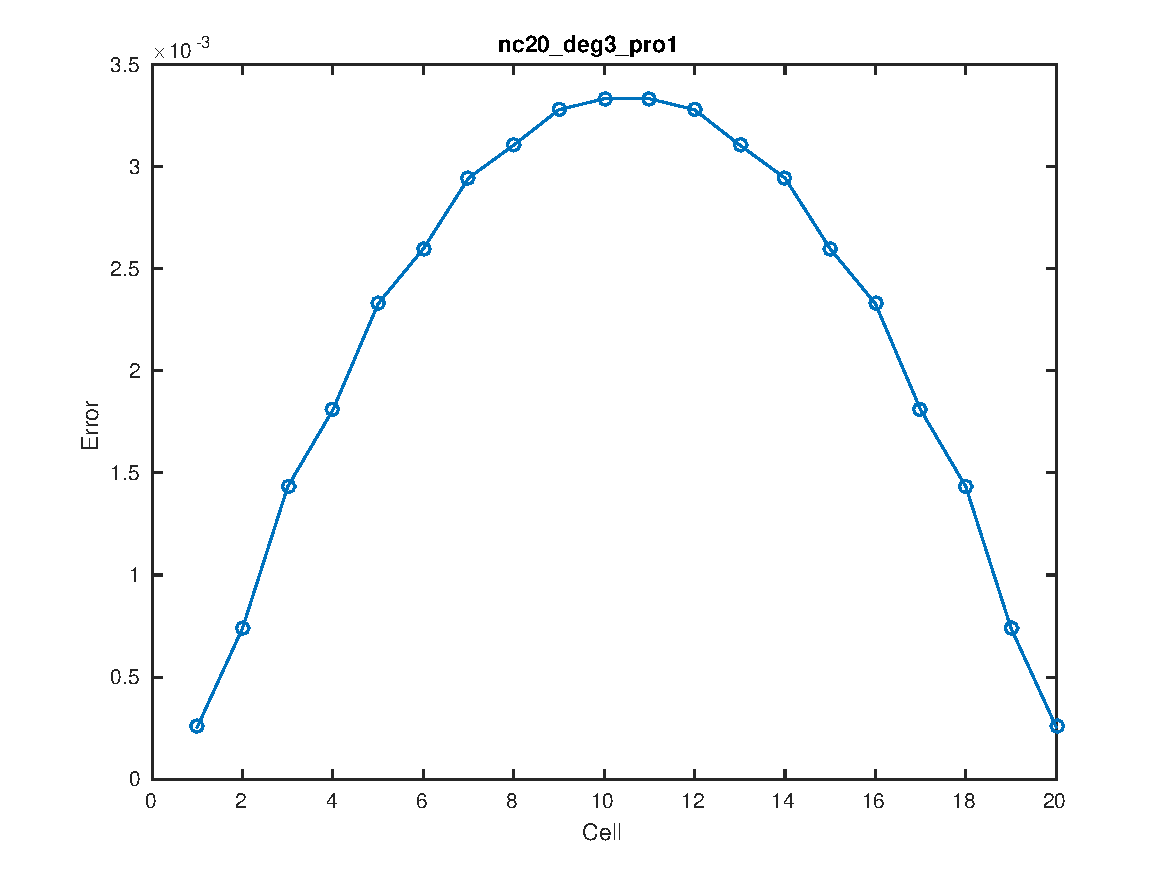
\includegraphics[width=\linewidth]{../../tests_01_01/test_01_01_test9_pro1/output/plots/nc20_deg3_wei111_pro1.pdf}
\end{subfigure}\hspace*{\fill}
\begin{subfigure}[b]{0.48\textwidth}
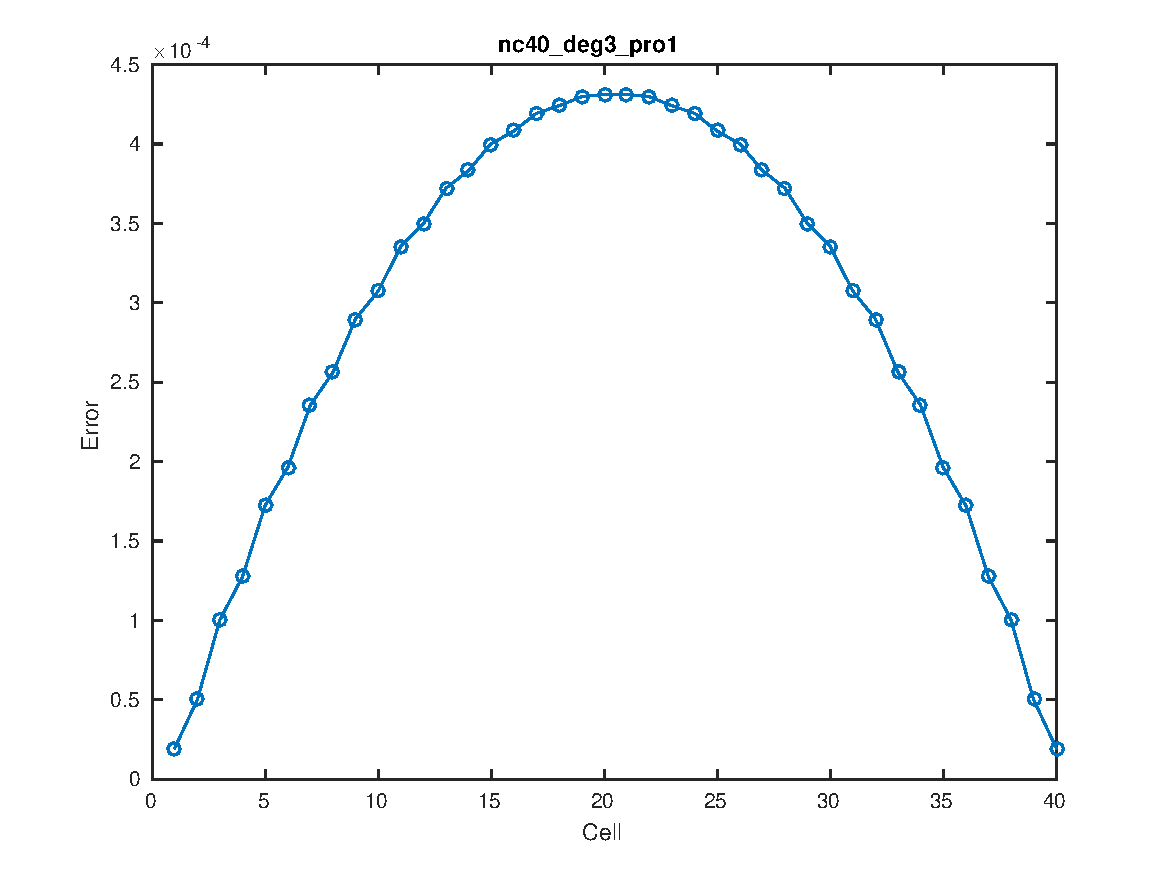
\includegraphics[width=\linewidth]{../../tests_01_01/test_01_01_test9_pro1/output/plots/nc40_deg3_wei111_pro1.pdf}
\end{subfigure}

\medskip
\begin{subfigure}[b]{0.48\textwidth}
\includegraphics[width=\linewidth]{../../tests_01_01/test_01_01_test9_pro1/output/plots/nc80_deg3_wei111_pro1.pdf}
\end{subfigure}\hspace*{\fill}
\begin{subfigure}[b]{0.48\textwidth}
\includegraphics[width=\linewidth]{../../tests_01_01/test_01_01_test9_pro1/output/plots/nc160_deg3_wei111_pro1.pdf}
\end{subfigure}

\medskip
\begin{subfigure}[b]{0.48\textwidth}
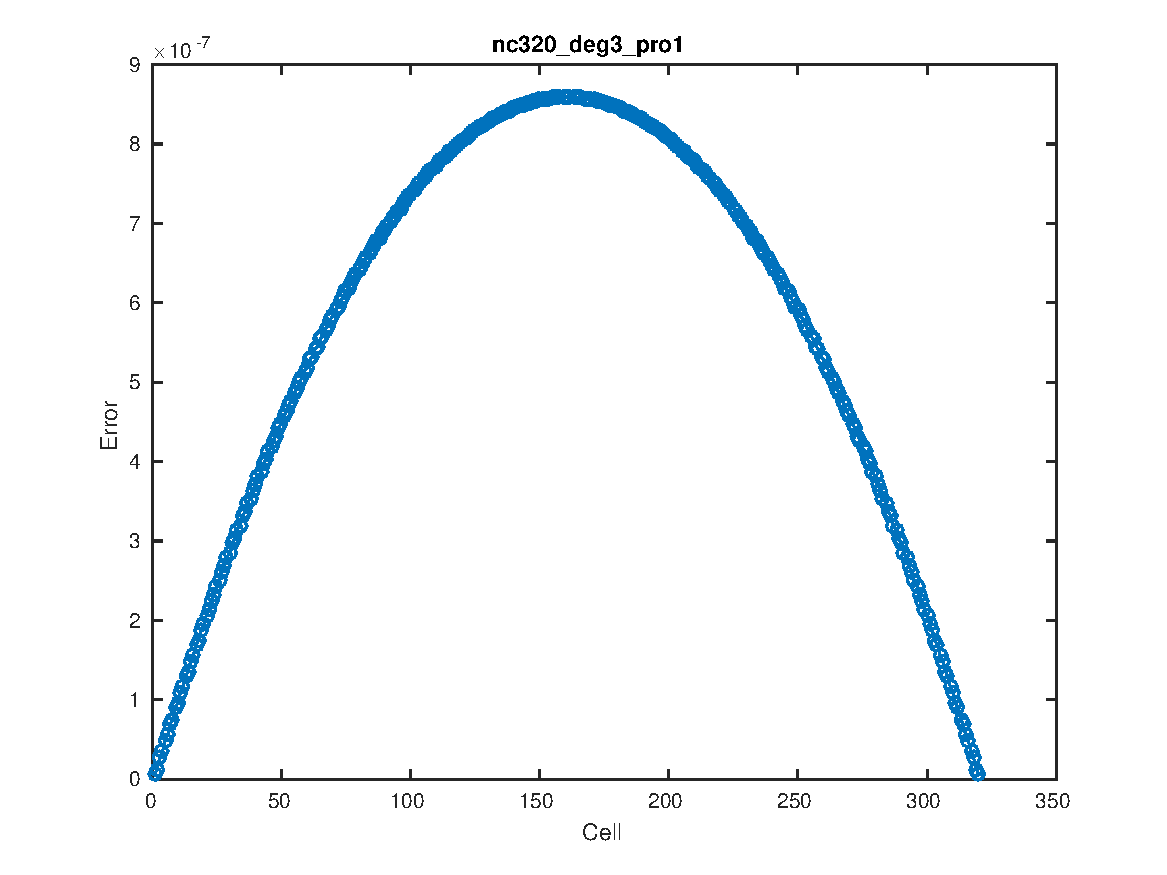
\includegraphics[width=\linewidth]{../../tests_01_01/test_01_01_test9_pro1/output/plots/nc320_deg3_wei111_pro1.pdf}
\end{subfigure}\hspace*{\fill}
\begin{subfigure}[b]{0.48\textwidth}
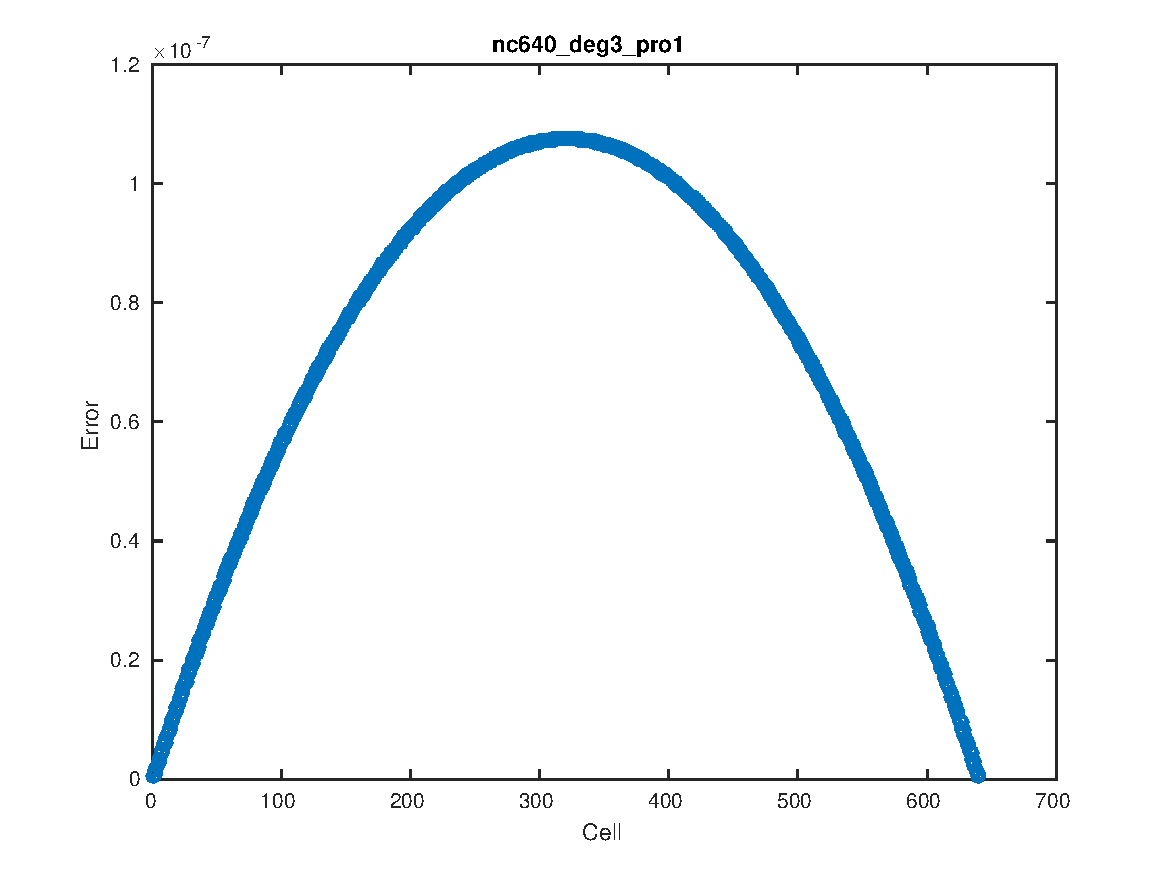
\includegraphics[width=\linewidth]{../../tests_01_01/test_01_01_test9_pro1/output/plots/nc640_deg3_wei111_pro1.pdf}
\end{subfigure}

\caption{$\omega=1|1,1$, d=3}
\end{figure}
%%%% 2
\begin{figure}[H]
\begin{subfigure}[b]{0.48\textwidth}
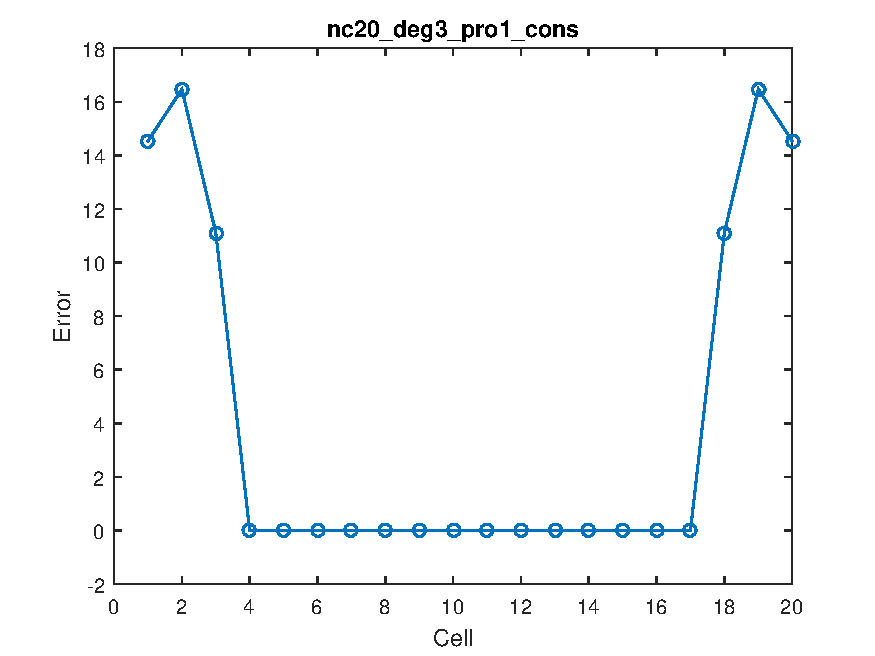
\includegraphics[width=\linewidth]{../../tests_01_01/test_01_01_test9_pro1_cons/output/plots/nc20_deg3_wei111_pro1_cons.pdf}
\end{subfigure}\hspace*{\fill}
\begin{subfigure}[b]{0.48\textwidth}
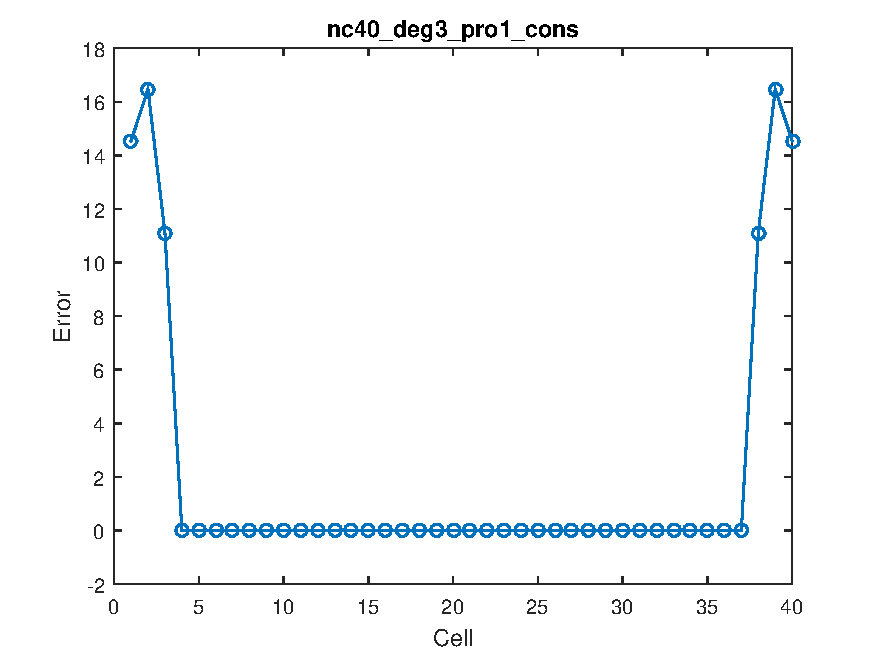
\includegraphics[width=\linewidth]{../../tests_01_01/test_01_01_test9_pro1_cons/output/plots/nc40_deg3_wei111_pro1_cons.pdf}
\end{subfigure}

\medskip
\begin{subfigure}[b]{0.48\textwidth}
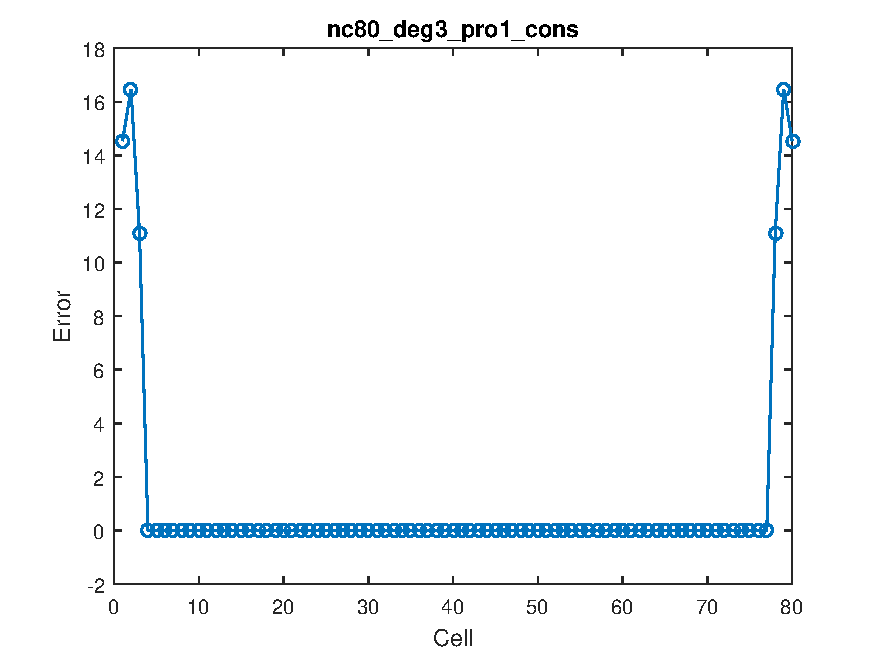
\includegraphics[width=\linewidth]{../../tests_01_01/test_01_01_test9_pro1_cons/output/plots/nc80_deg3_wei111_pro1_cons.pdf}
\end{subfigure}\hspace*{\fill}
\begin{subfigure}[b]{0.48\textwidth}
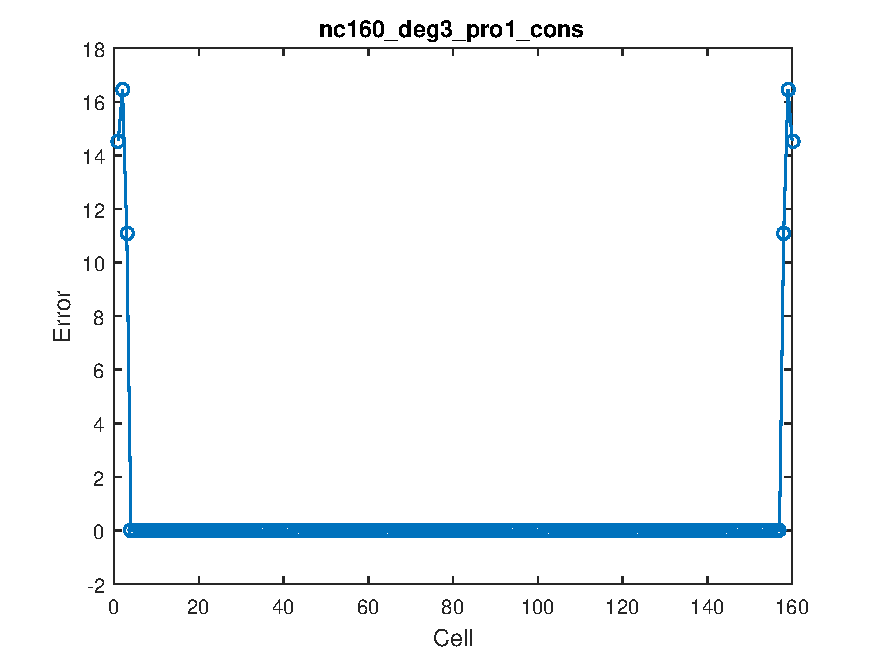
\includegraphics[width=\linewidth]{../../tests_01_01/test_01_01_test9_pro1_cons/output/plots/nc160_deg3_wei111_pro1_cons.pdf}
\end{subfigure}

\medskip
\begin{subfigure}[b]{0.48\textwidth}
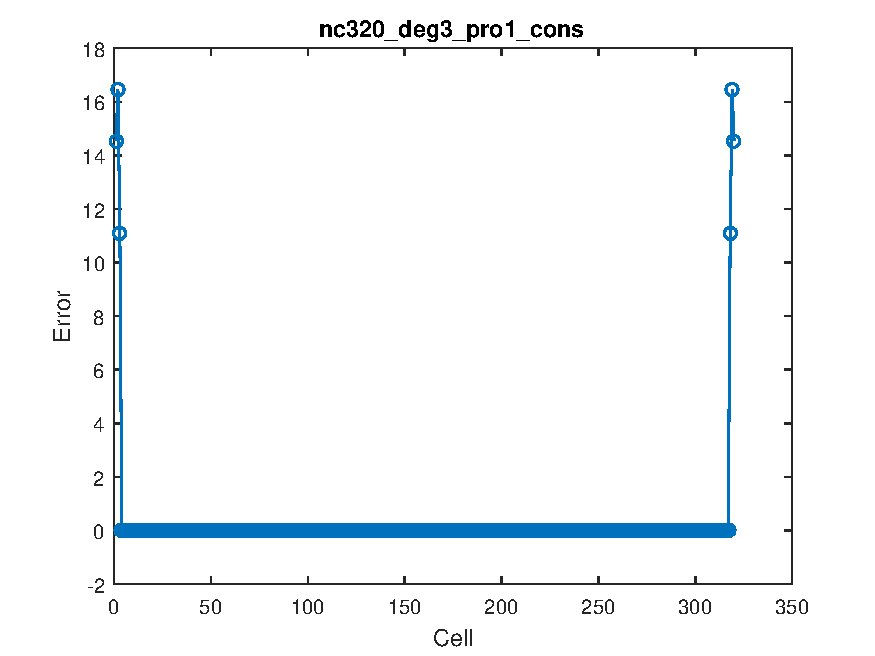
\includegraphics[width=\linewidth]{../../tests_01_01/test_01_01_test9_pro1_cons/output/plots/nc320_deg3_wei111_pro1_cons.pdf}
\end{subfigure}\hspace*{\fill}
\begin{subfigure}[b]{0.48\textwidth}
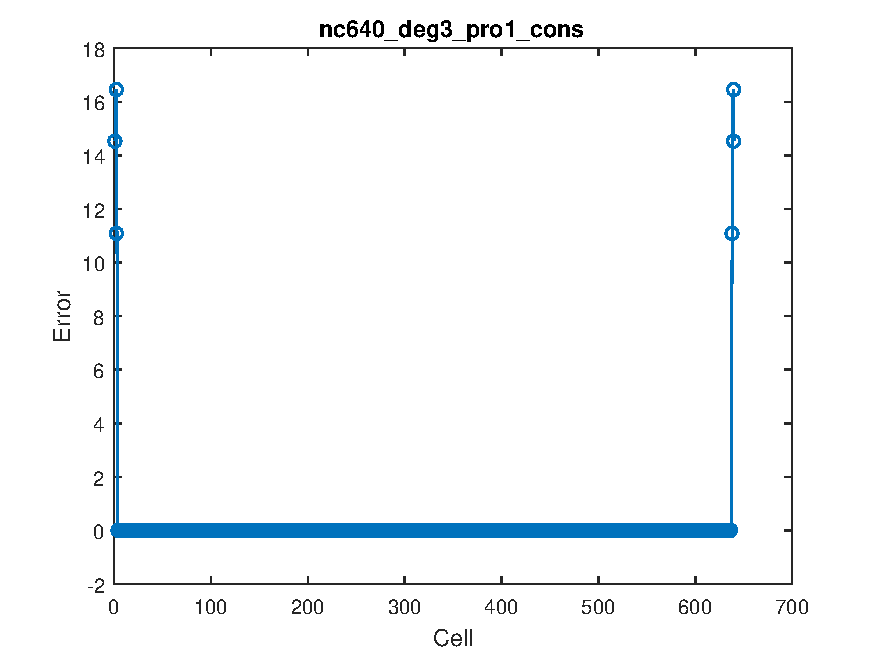
\includegraphics[width=\linewidth]{../../tests_01_01/test_01_01_test9_pro1_cons/output/plots/nc640_deg3_wei111_pro1_cons.pdf}
\end{subfigure}

\caption{$\omega=1|1,1$, d=3 (consistency)}
\end{figure}
%%%% 3
\begin{figure}[H]
\begin{subfigure}[b]{0.48\textwidth}
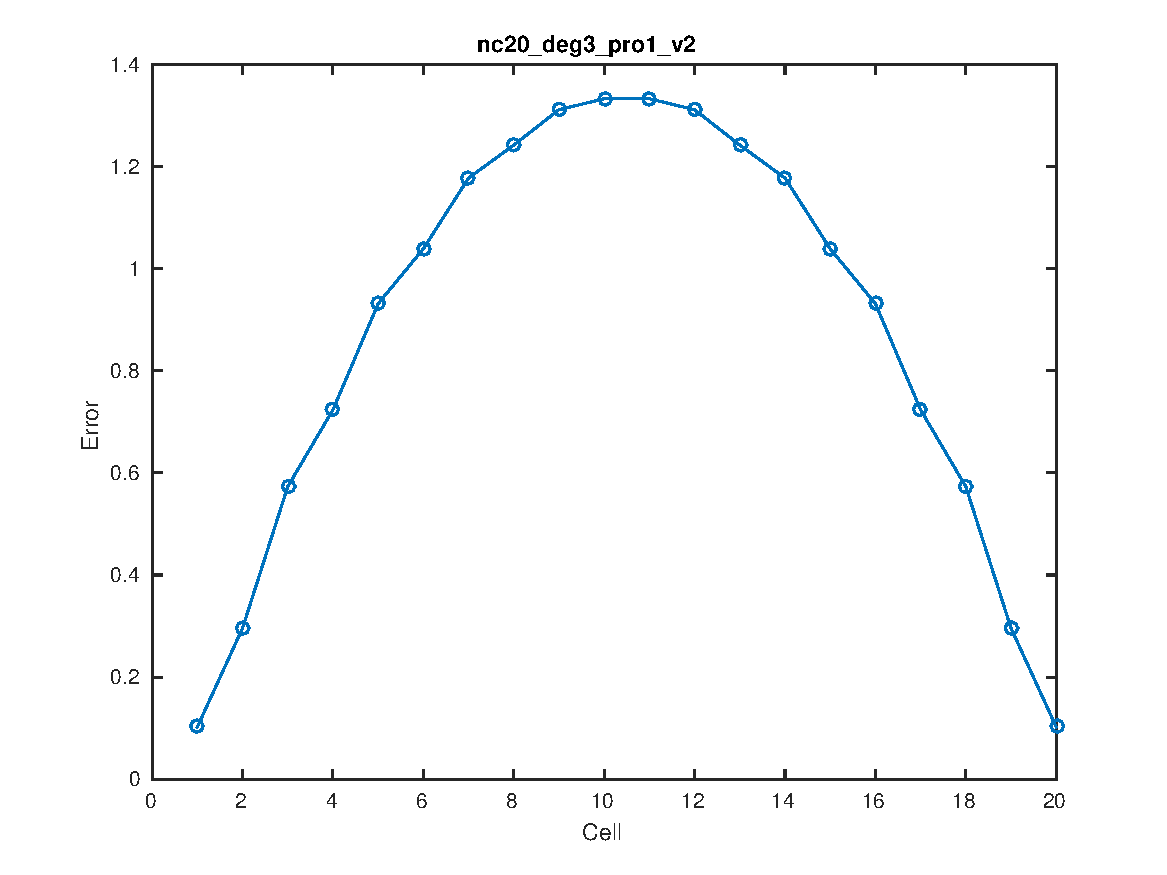
\includegraphics[width=\linewidth]{../../tests_01_01/test_01_01_test9_pro1/output/plots/nc20_deg3_wei111_pro1_v2.pdf}
\end{subfigure}\hspace*{\fill}
\begin{subfigure}[b]{0.48\textwidth}
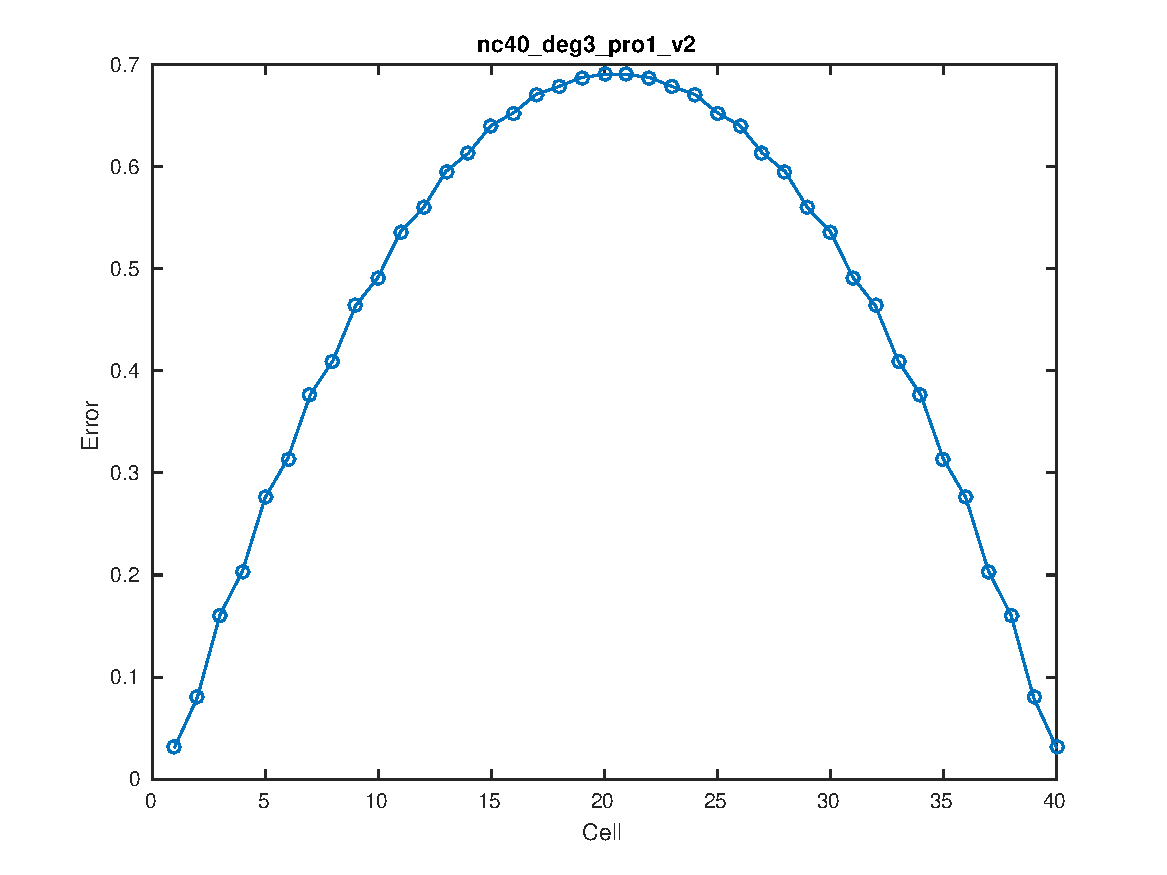
\includegraphics[width=\linewidth]{../../tests_01_01/test_01_01_test9_pro1/output/plots/nc40_deg3_wei111_pro1_v2.pdf}
\end{subfigure}

\medskip
\begin{subfigure}[b]{0.48\textwidth}
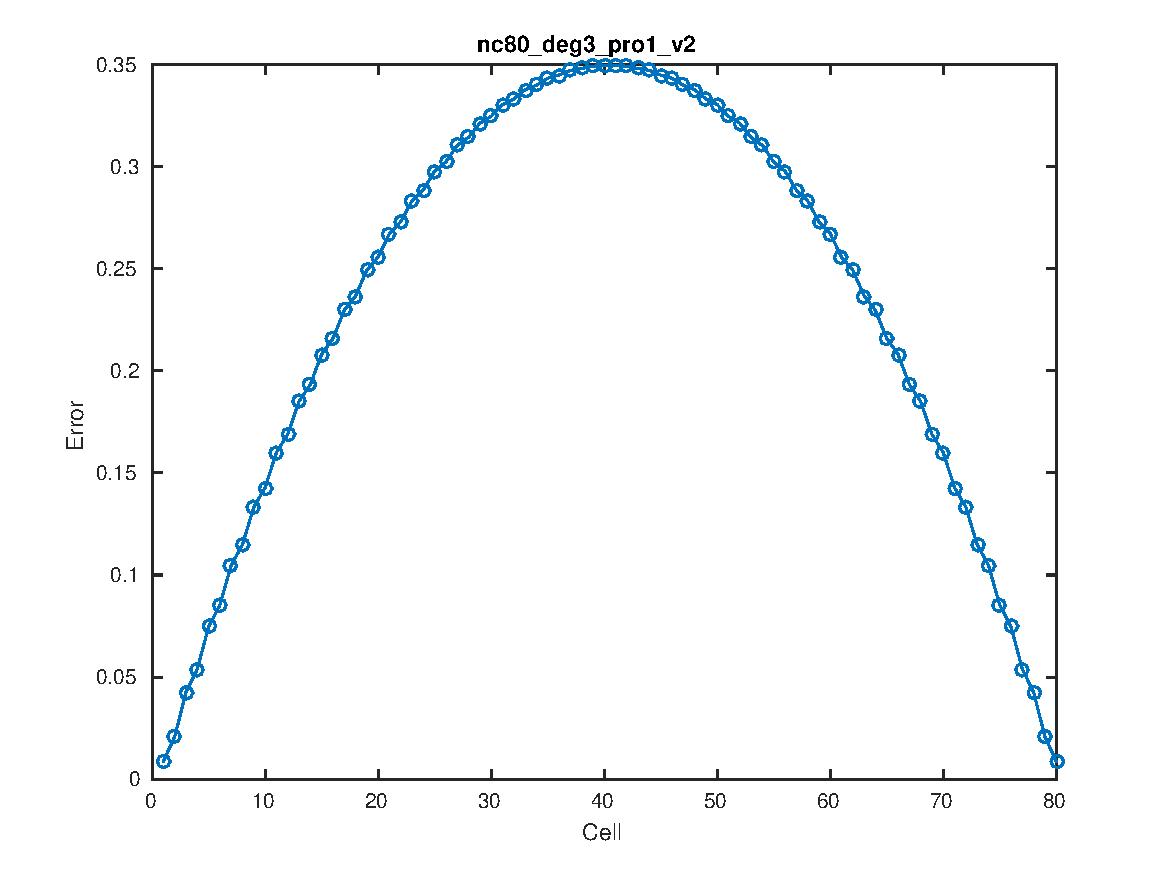
\includegraphics[width=\linewidth]{../../tests_01_01/test_01_01_test9_pro1/output/plots/nc80_deg3_wei111_pro1_v2.pdf}
\end{subfigure}\hspace*{\fill}
\begin{subfigure}[b]{0.48\textwidth}
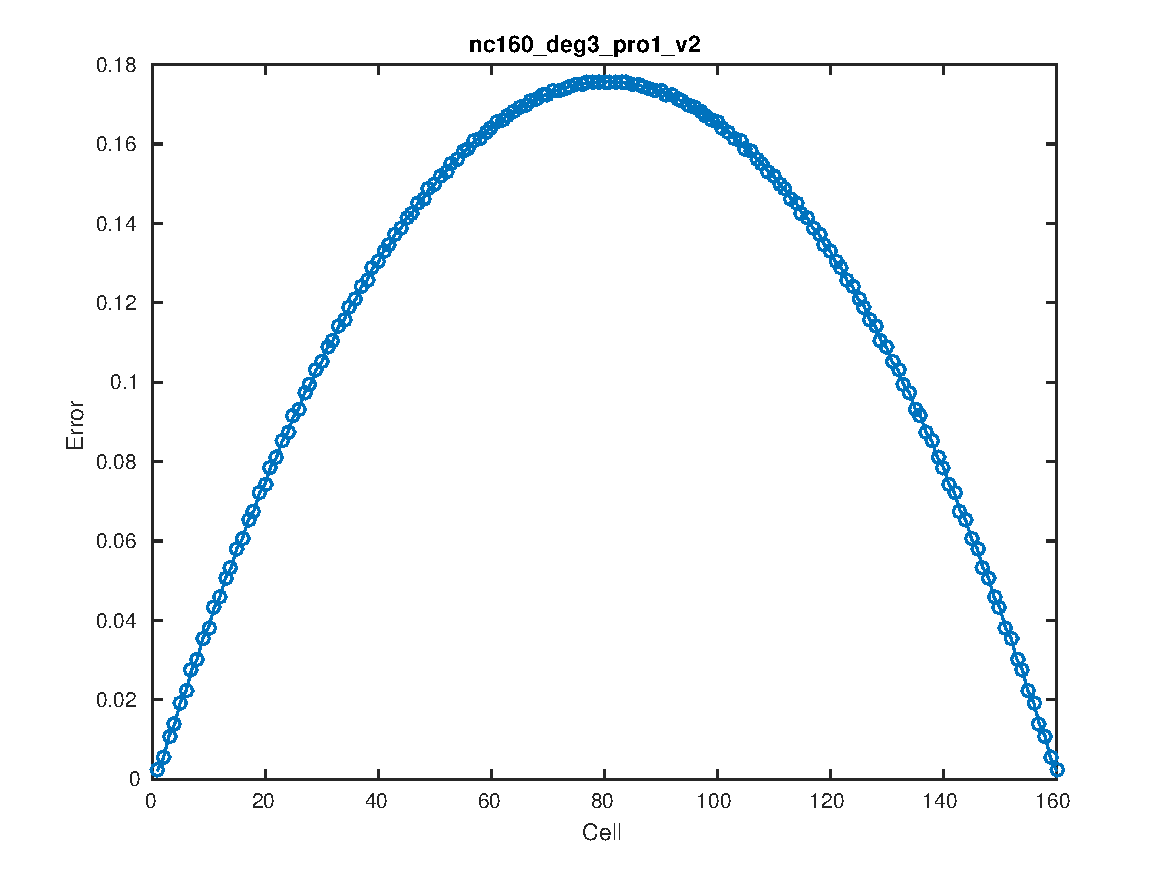
\includegraphics[width=\linewidth]{../../tests_01_01/test_01_01_test9_pro1/output/plots/nc160_deg3_wei111_pro1_v2.pdf}
\end{subfigure}

\medskip
\begin{subfigure}[b]{0.48\textwidth}
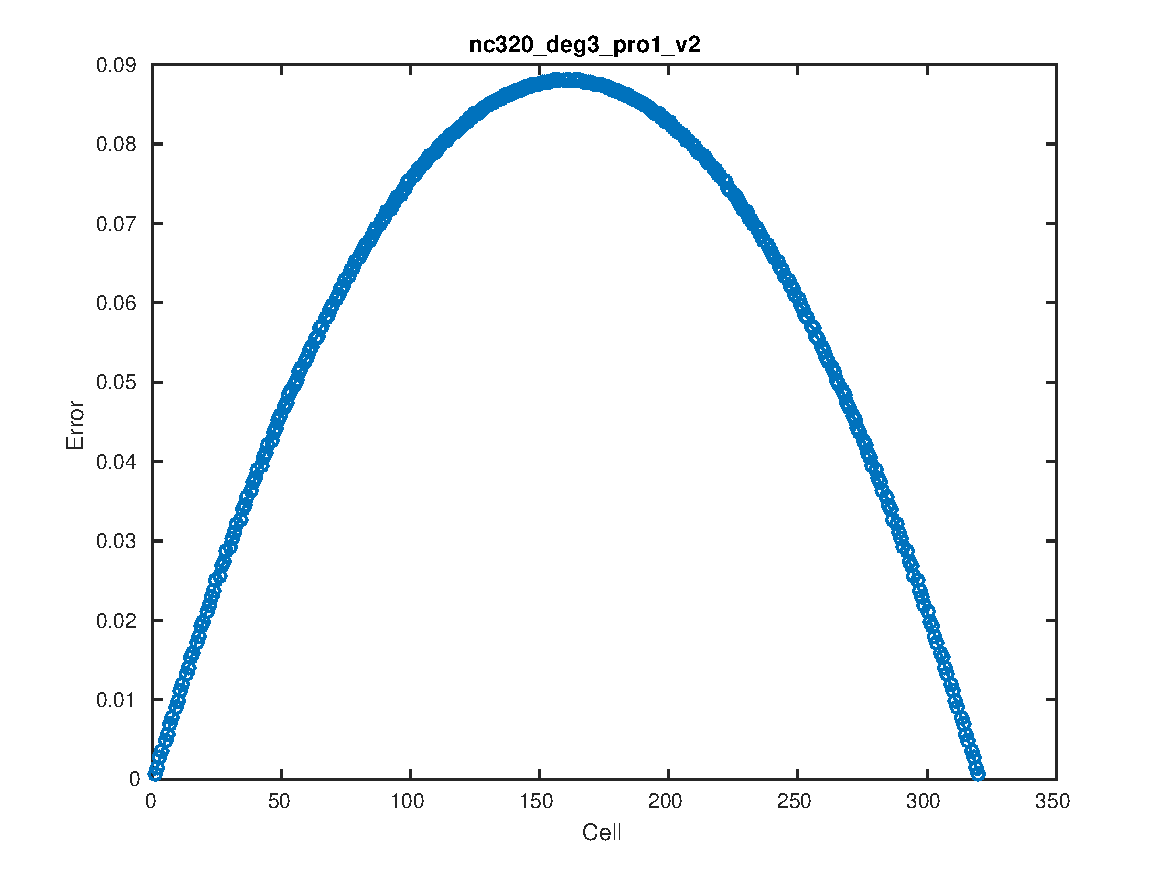
\includegraphics[width=\linewidth]{../../tests_01_01/test_01_01_test9_pro1/output/plots/nc320_deg3_wei111_pro1_v2.pdf}
\end{subfigure}\hspace*{\fill}
\begin{subfigure}[b]{0.48\textwidth}
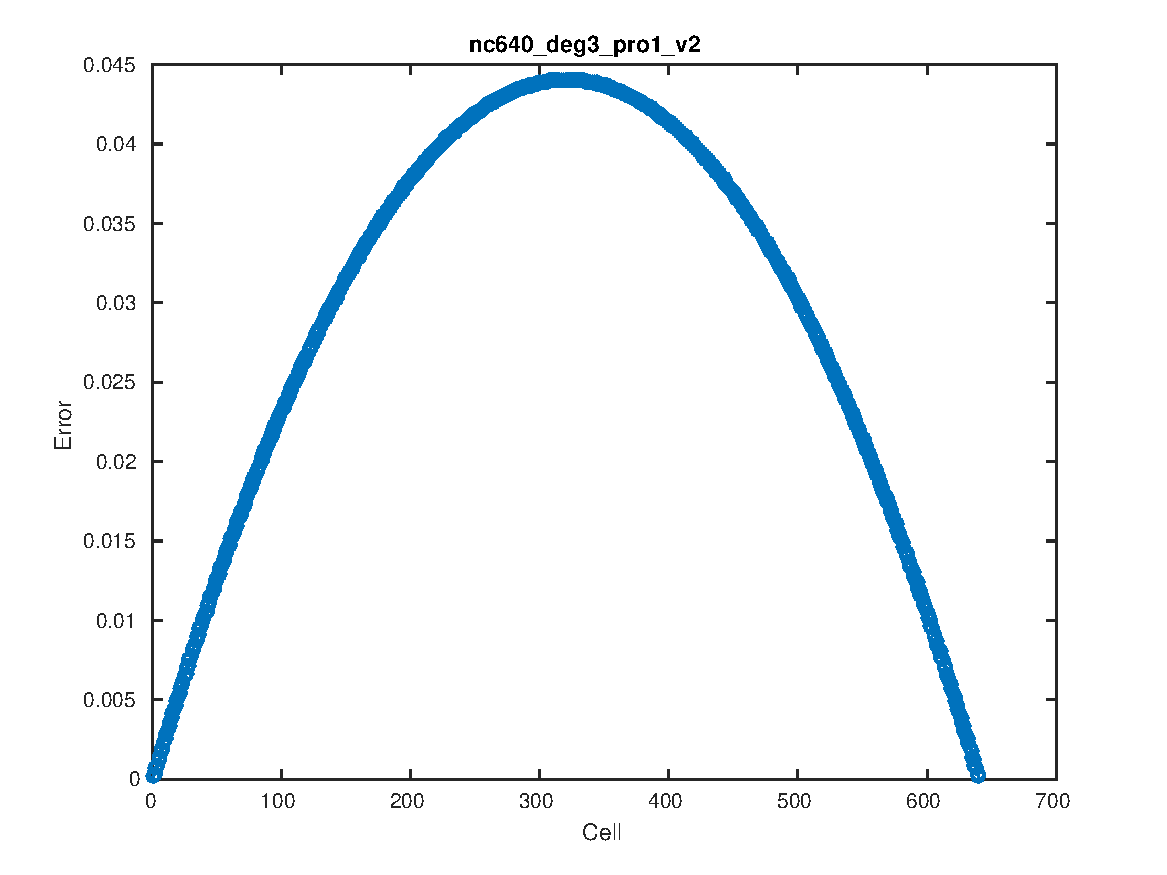
\includegraphics[width=\linewidth]{../../tests_01_01/test_01_01_test9_pro1/output/plots/nc640_deg3_wei111_pro1_v2.pdf}
\end{subfigure}

\caption{$\omega=1|1,1$, d=3  $\left(\frac{x-\overline{x}}{h^2}\right)$}
\end{figure}

%%%%%%%%%%%%%%%%%%%%%
\pagebreak
In this tests we consider:
\begin{itemize}
\item $\psi(x)=x^4$
\item $\psi_\text l=0$
\item $\psi_\text r=1$
\item $\psi_\text{ll}=0$
\item $\psi_\text{rr}=4$
\item $g(x)=-24$
\item non-constant mesh
\end{itemize}
\begin{table}[H]
\caption{(normal)}
\setlength{\tabcolsep}{5pt}
\centering
\begin{tabular}{@{}l c c c@{}}
\toprule
 &  & \multicolumn{2}{c}{PRO1}\\
\midrule
 & $I$ & E$_{0,I}(E_{\infty})$ & E$_{0,I}(O_{\infty})$\\
\midrule
\multirow{6}{*}{$\mathbb{P}_{3}$}
 & 20 & 5.11E$-$03 & ---\\
 & 40 & 1.55E$-$03 & 1.72\\
 & 80 & 4.27E$-$04 & 1.86\\
 & 160 & 1.06E$-$04 & 2.02\\
 & 320 & 2.45E$-$05 & 2.11\\
 & 640 & 1.32E$-$05 & 0.90\\
\midrule
\multirow{6}{*}{$\mathbb{P}_{5}$}
 & 20 & 5.05E$-$14 & ---\\
 & 40 & 4.53E$-$13 & $\uparrow$\\
 & 80 & 6.40E$-$13 & $\uparrow$\\
 & 160 & 2.51E$-$12 & $\uparrow$\\
 & 320 & 1.38E$-$11 & $\uparrow$\\
 & 640 & 7.04E$-$10 & $\uparrow$\\
\bottomrule
\end{tabular}
\label{Table:PRO:test_01_01_test48_pro1}
\end{table}

\begin{table}[H]
\caption{(consistency)}
\setlength{\tabcolsep}{5pt}
\centering
\begin{tabular}{@{}l c c c@{}}
\toprule
 &  & \multicolumn{2}{c}{PRO1}\\
\midrule
 & $I$ & E$_{0,I}(E_{\infty})$ & E$_{0,I}(O_{\infty})$\\
\midrule
\multirow{6}{*}{$\mathbb{P}_{3}$}
 & 20 & 2.00E$+$01 & ---\\
 & 40 & 2.00E$+$01 & $\uparrow$\\
 & 80 & 2.00E$+$01 & $\uparrow$\\
 & 160 & 2.00E$+$01 & $\uparrow$\\
 & 320 & 2.00E$+$01 & $\uparrow$\\
 & 640 & 2.00E$+$01 & $\uparrow$\\
\midrule
\multirow{6}{*}{$\mathbb{P}_{5}$}
 & 20 & 4.72E$-$09 & ---\\
 & 40 & 2.17E$-$07 & $\uparrow$\\
 & 80 & 2.43E$-$07 & $\uparrow$\\
 & 160 & 5.00E$-$06 & $\uparrow$\\
 & 320 & 1.69E$-$04 & $\uparrow$\\
 & 640 & 4.07E$-$03 & $\uparrow$\\
\bottomrule
\end{tabular}
\label{Table:PRO:test_01_01_test48_pro1}
\end{table}


\begin{figure}[H]
\begin{subfigure}[b]{0.48\textwidth}
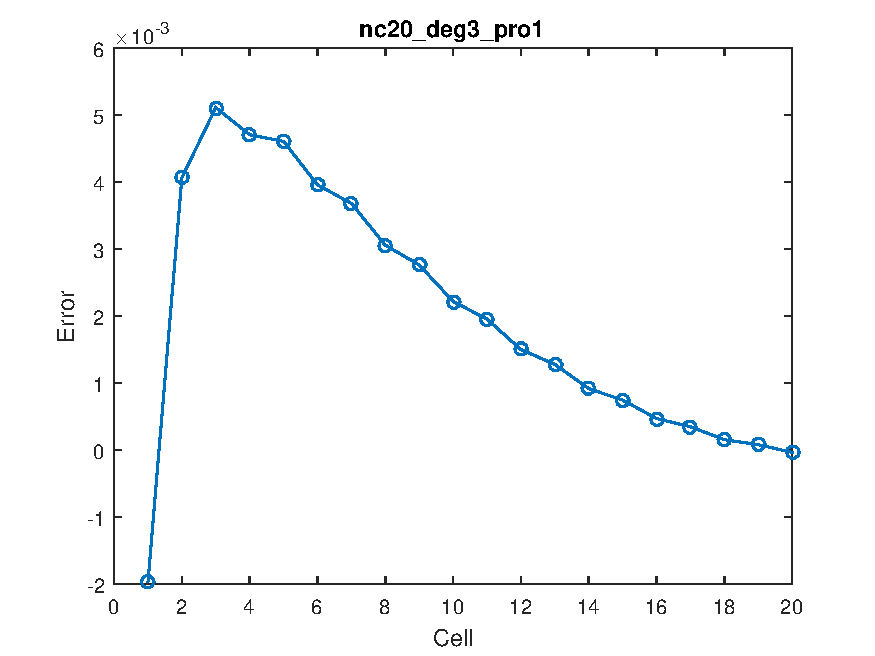
\includegraphics[width=\linewidth]{../../tests_01_01/test_01_01_test48_pro1/output/plots/nc20_deg3_wei111_pro1.pdf}
\end{subfigure}\hspace*{\fill}
\begin{subfigure}[b]{0.48\textwidth}
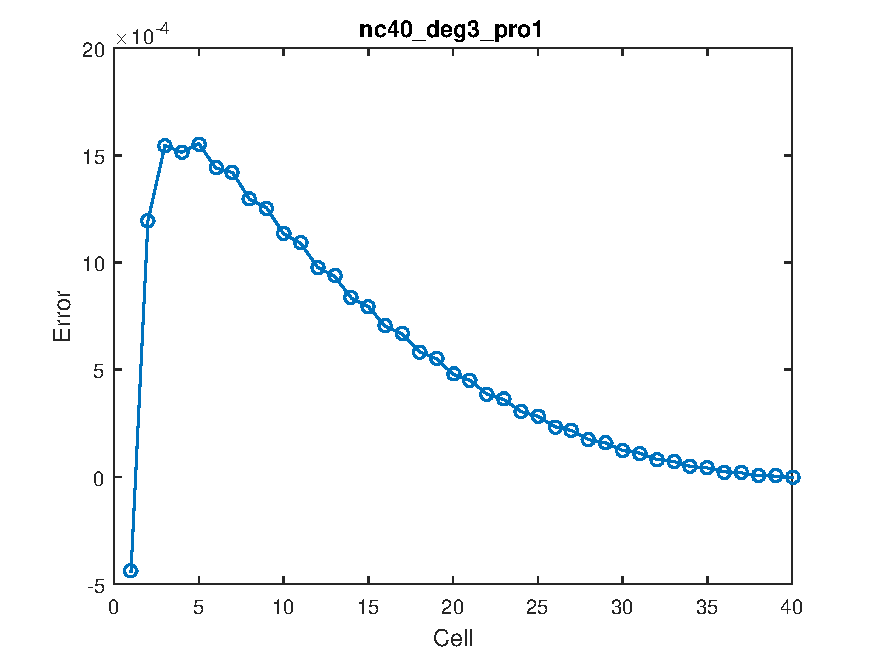
\includegraphics[width=\linewidth]{../../tests_01_01/test_01_01_test48_pro1/output/plots/nc40_deg3_wei111_pro1.pdf}
\end{subfigure}

\medskip
\begin{subfigure}[b]{0.48\textwidth}
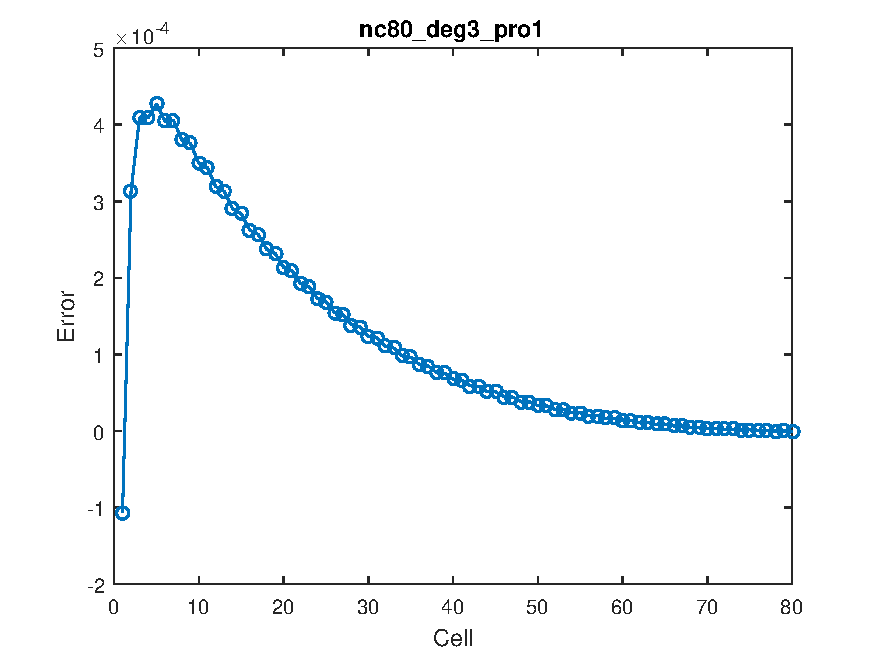
\includegraphics[width=\linewidth]{../../tests_01_01/test_01_01_test48_pro1/output/plots/nc80_deg3_wei111_pro1.pdf}
\end{subfigure}\hspace*{\fill}
\begin{subfigure}[b]{0.48\textwidth}
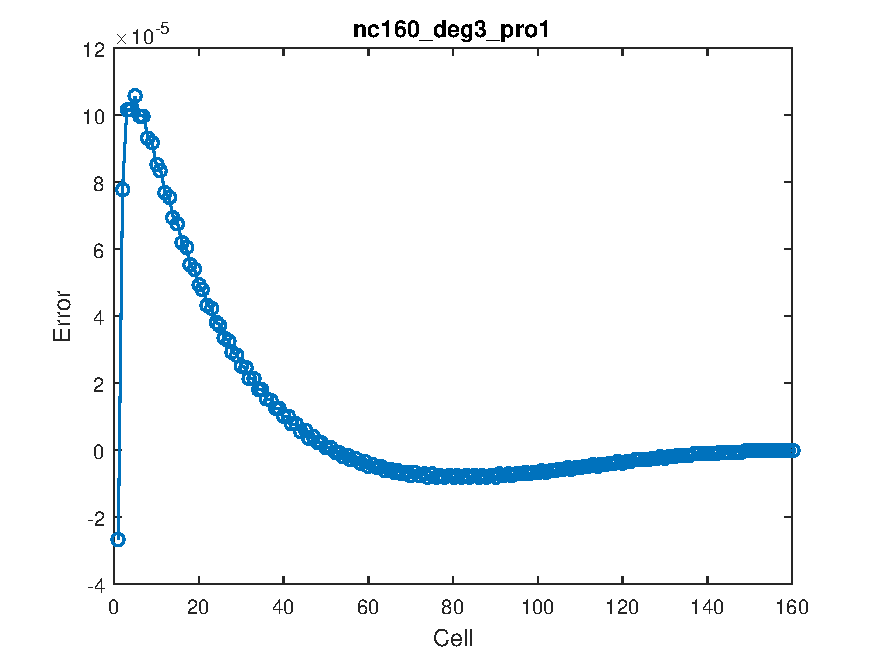
\includegraphics[width=\linewidth]{../../tests_01_01/test_01_01_test48_pro1/output/plots/nc160_deg3_wei111_pro1.pdf}
\end{subfigure}

\medskip
\begin{subfigure}[b]{0.48\textwidth}
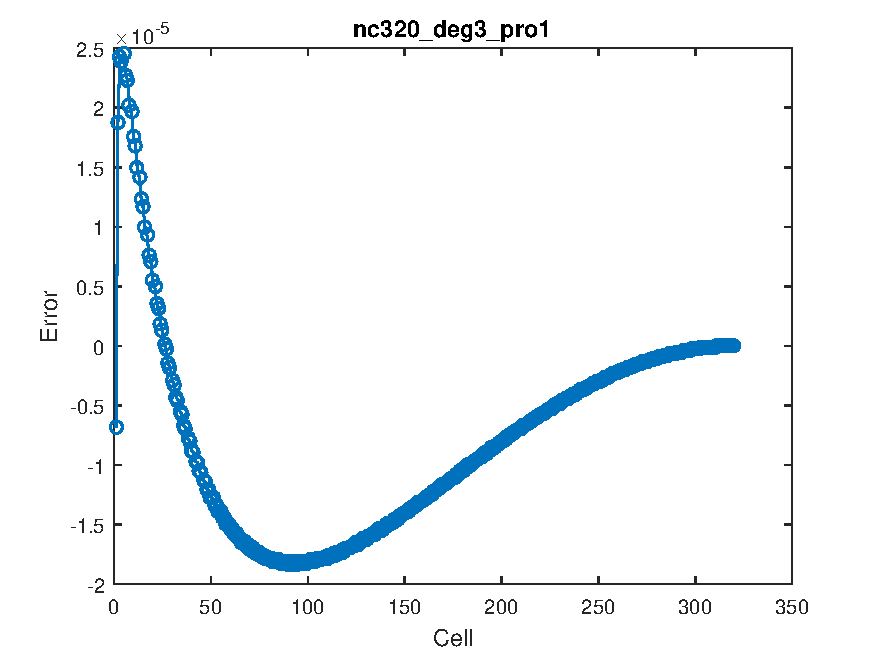
\includegraphics[width=\linewidth]{../../tests_01_01/test_01_01_test48_pro1/output/plots/nc320_deg3_wei111_pro1.pdf}
\end{subfigure}\hspace*{\fill}
\begin{subfigure}[b]{0.48\textwidth}
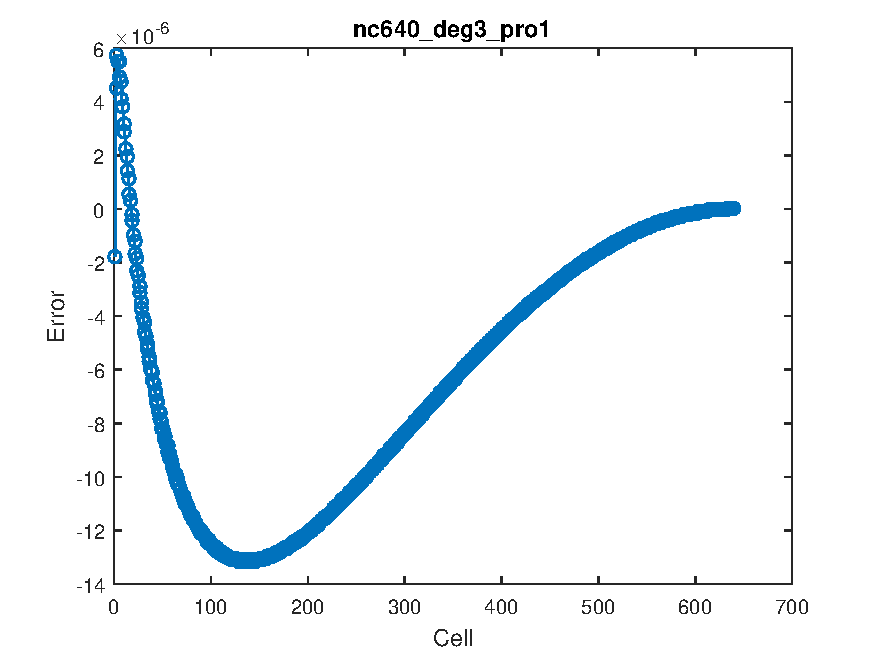
\includegraphics[width=\linewidth]{../../tests_01_01/test_01_01_test48_pro1/output/plots/nc640_deg3_wei111_pro1.pdf}
\end{subfigure}

\caption{$\omega=1|1,1$, d=3}
\end{figure}
%%%% 2
\begin{figure}[H]
\begin{subfigure}[b]{0.48\textwidth}
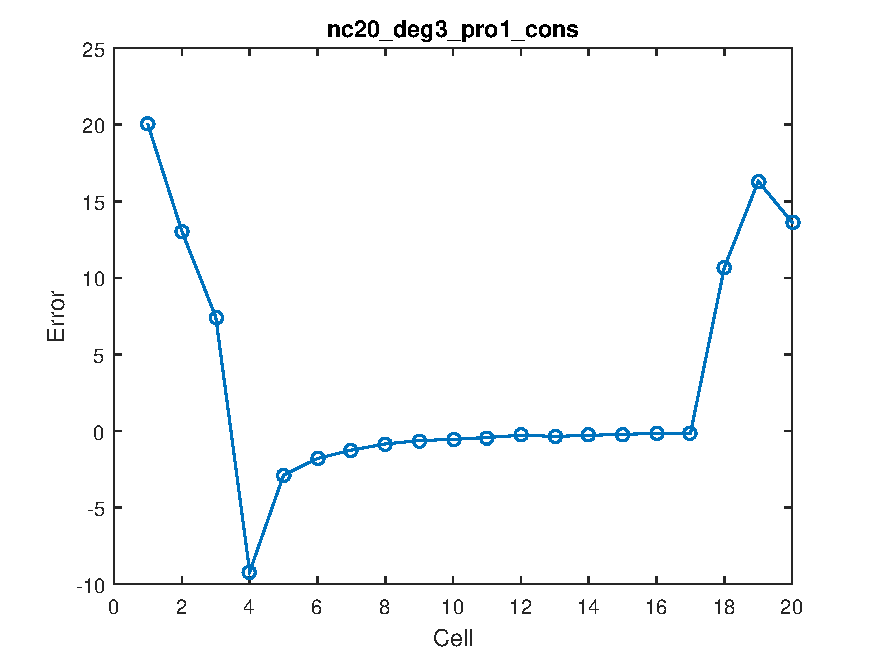
\includegraphics[width=\linewidth]{../../tests_01_01/test_01_01_test48_pro1_cons/output/plots/nc20_deg3_wei111_pro1_cons.pdf}
\end{subfigure}\hspace*{\fill}
\begin{subfigure}[b]{0.48\textwidth}
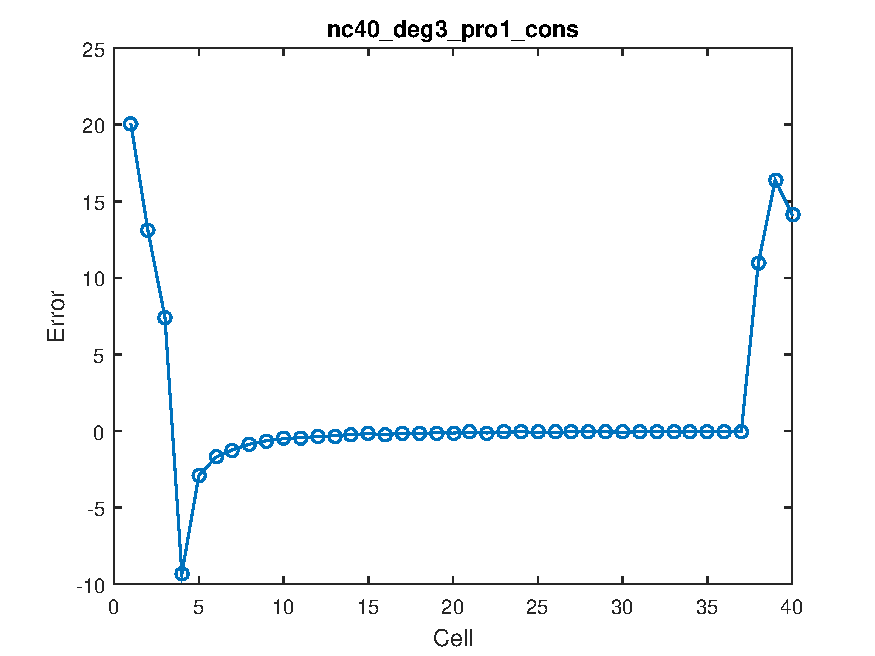
\includegraphics[width=\linewidth]{../../tests_01_01/test_01_01_test48_pro1_cons/output/plots/nc40_deg3_wei111_pro1_cons.pdf}
\end{subfigure}

\medskip
\begin{subfigure}[b]{0.48\textwidth}
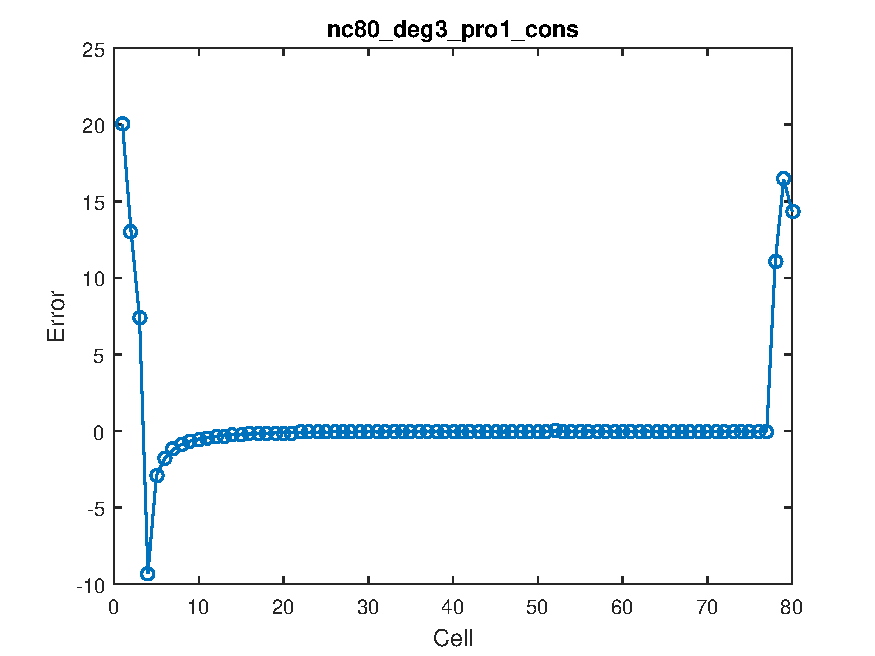
\includegraphics[width=\linewidth]{../../tests_01_01/test_01_01_test48_pro1_cons/output/plots/nc80_deg3_wei111_pro1_cons.pdf}
\end{subfigure}\hspace*{\fill}
\begin{subfigure}[b]{0.48\textwidth}
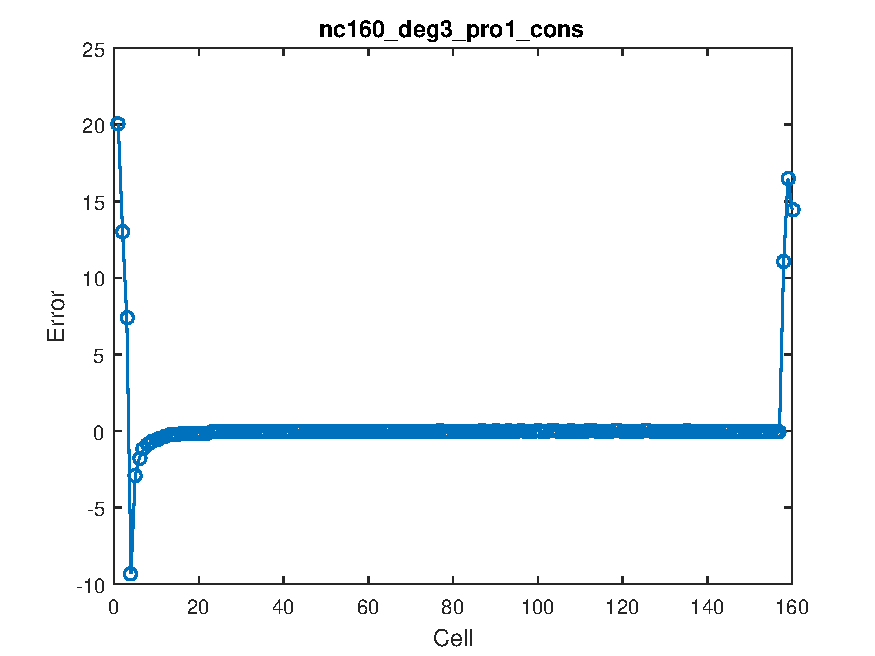
\includegraphics[width=\linewidth]{../../tests_01_01/test_01_01_test48_pro1_cons/output/plots/nc160_deg3_wei111_pro1_cons.pdf}
\end{subfigure}

\medskip
\begin{subfigure}[b]{0.48\textwidth}
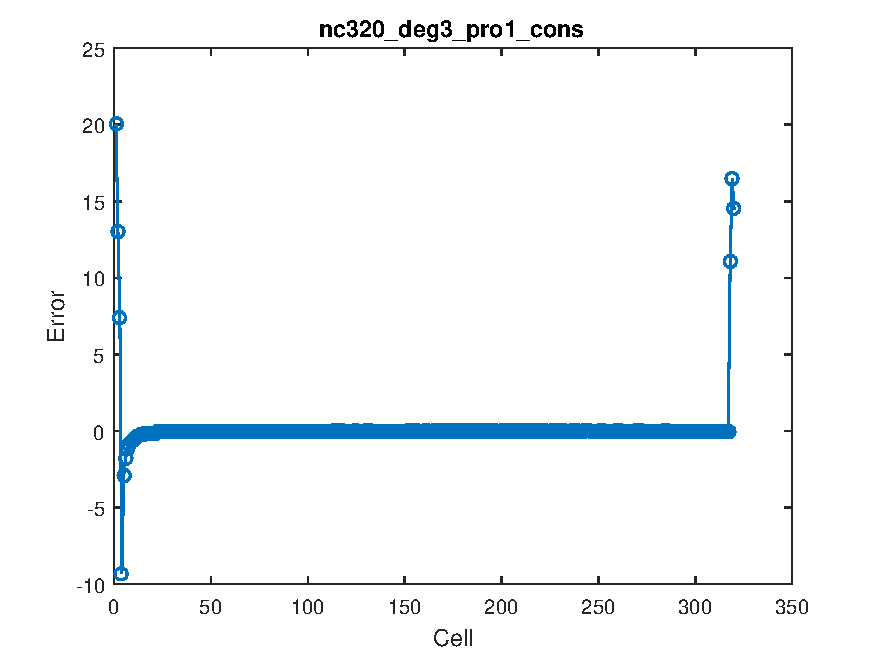
\includegraphics[width=\linewidth]{../../tests_01_01/test_01_01_test48_pro1_cons/output/plots/nc320_deg3_wei111_pro1_cons.pdf}
\end{subfigure}\hspace*{\fill}
\begin{subfigure}[b]{0.48\textwidth}
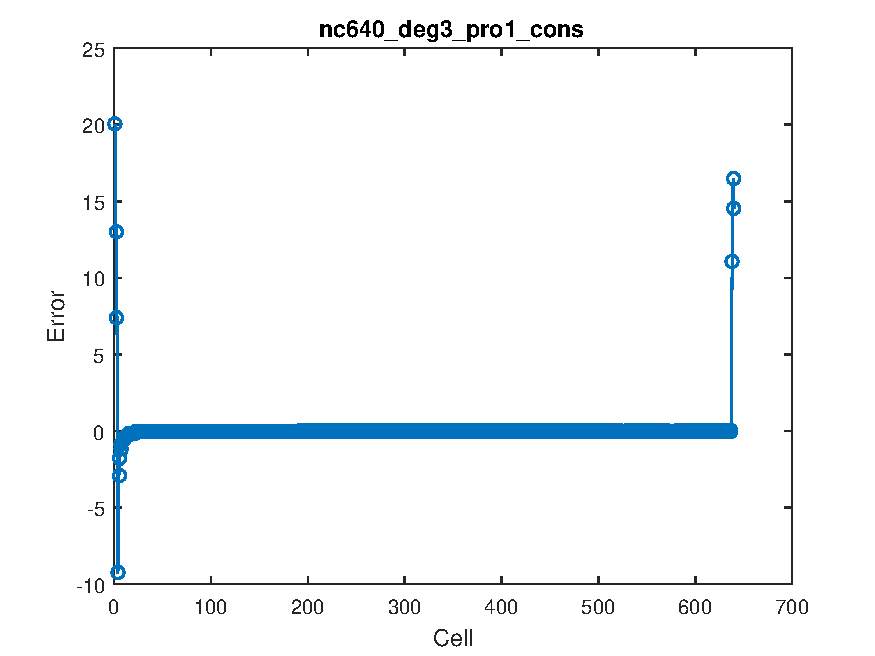
\includegraphics[width=\linewidth]{../../tests_01_01/test_01_01_test48_pro1_cons/output/plots/nc640_deg3_wei111_pro1_cons.pdf}
\end{subfigure}

\caption{$\omega=1|1,1$, d=3 (consistency)}
\end{figure}

\begin{figure}[H]
\centering
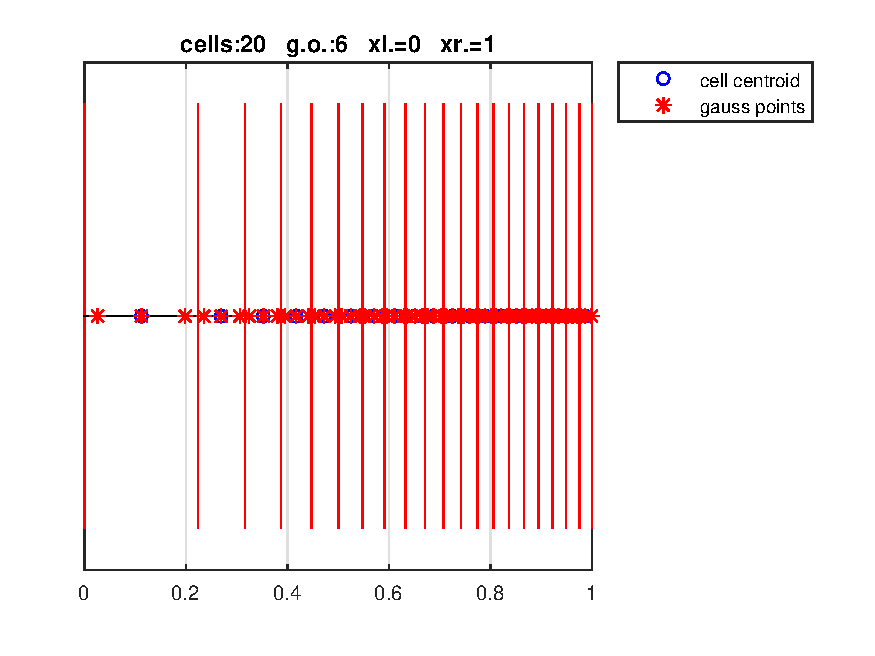
\includegraphics[width=.8\textwidth]{../../tests_01_01/test_01_01_test48_pro1_cons/output/plots/mesh.pdf}
\caption{Non-constant mesh.}
\end{figure}
\pagebreak

%%%%%%%%%%%%%%%%%%%%%
\pagebreak
In this tests we consider:
\begin{itemize}
\item $\psi(x)=x^4$
\item $\psi_\text l=0$
\item $\psi_\text r=1$
\item $\psi_\text{ll}=0$
\item $\psi_\text{rr}=4$
\item $g(x)=-24$
\item constant mesh
\item 
\end{itemize}
\begin{table}[H]
\caption{(normal)}
\setlength{\tabcolsep}{5pt}
\centering
\begin{tabular}{@{}l c c c@{}}
\toprule
 &  & \multicolumn{2}{c}{PRO1}\\
\midrule
 & $I$ & E$_{0,I}(E_{\infty})$ & E$_{0,I}(O_{\infty})$\\
\midrule
\multirow{3}{*}{$\mathbb{P}_{3}$}
 & 20 & 8.31E$-$04 & ---\\
 & 40 & 3.74E$-$05 & 4.48\\
 & 80 & 1.32E$-$05 & 1.50\\
\midrule
\multirow{3}{*}{$\mathbb{P}_{5}$}
 & 20 & 2.45E$-$14 & ---\\
 & 40 & 1.16E$-$13 & $\uparrow$\\
 & 80 & 4.90E$-$13 & $\uparrow$\\
\bottomrule
\end{tabular}
\label{Table:PRO:test_01_01_test49_pro1}
\end{table}

\input{../../tests_01_01/test_01_01_test49_pro1_cons/output/tables/test_01_01_test49_pro1_cons.tex}

\begin{figure}[H]
\begin{subfigure}[b]{0.48\textwidth}
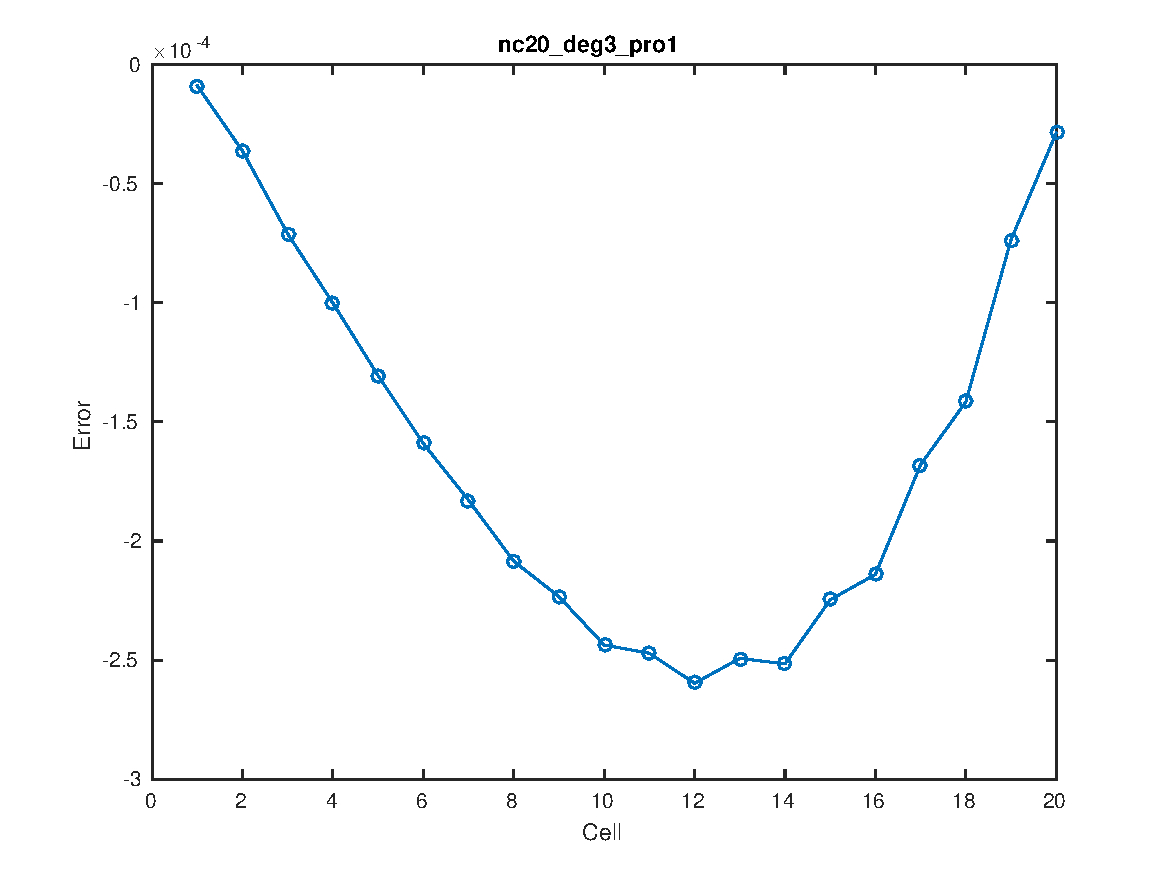
\includegraphics[width=\linewidth]{../../tests_01_01/test_01_01_test49_pro1/output/plots/nc20_deg3_wei111_pro1.pdf}
\end{subfigure}\hspace*{\fill}
\begin{subfigure}[b]{0.48\textwidth}
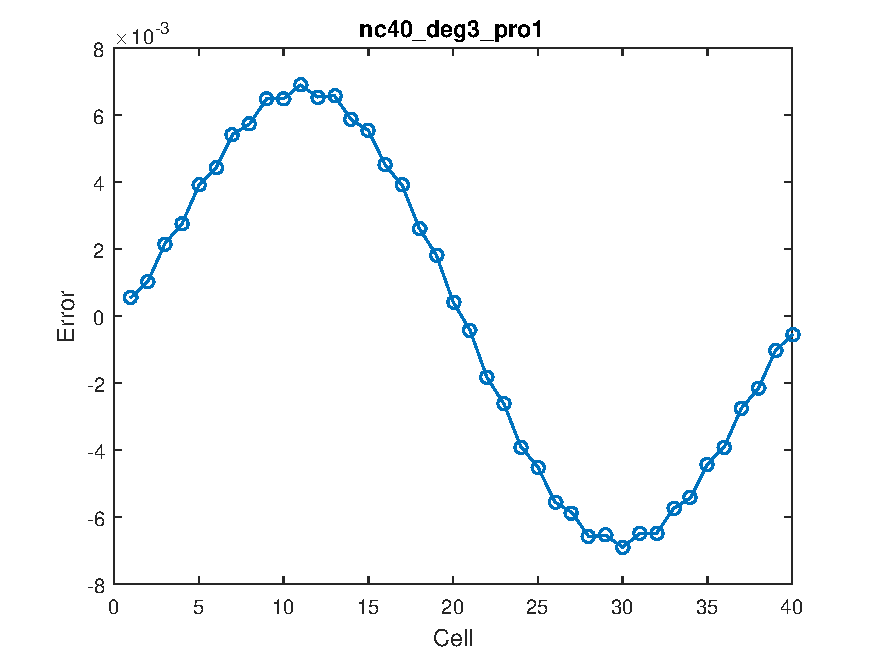
\includegraphics[width=\linewidth]{../../tests_01_01/test_01_01_test49_pro1/output/plots/nc40_deg3_wei111_pro1.pdf}
\end{subfigure}

\medskip
\begin{subfigure}[b]{0.48\textwidth}
\includegraphics[width=\linewidth]{../../tests_01_01/test_01_01_test49_pro1/output/plots/nc80_deg3_wei111_pro1.pdf}
\end{subfigure}\hspace*{\fill}
\begin{subfigure}[b]{0.48\textwidth}
\includegraphics[width=\linewidth]{../../tests_01_01/test_01_01_test49_pro1/output/plots/nc160_deg3_wei111_pro1.pdf}
\end{subfigure}

\medskip
\begin{subfigure}[b]{0.48\textwidth}
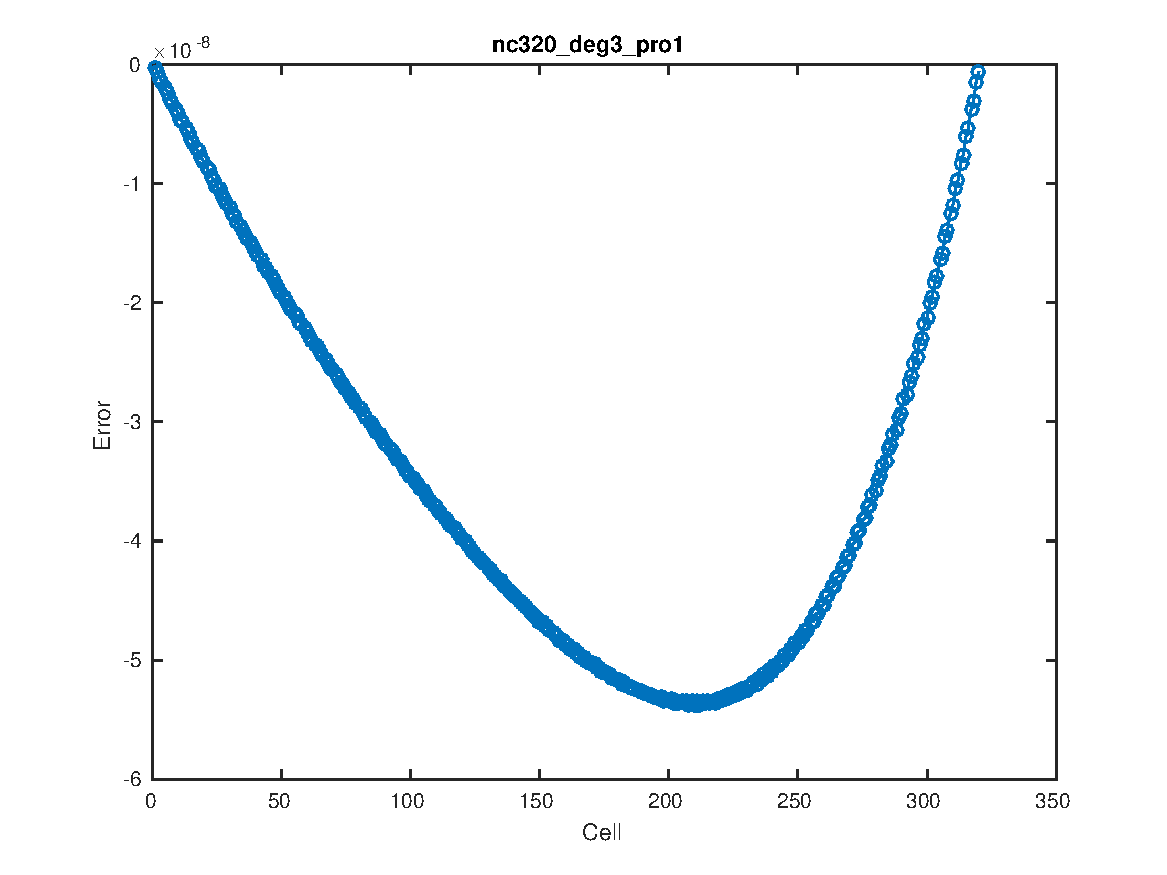
\includegraphics[width=\linewidth]{../../tests_01_01/test_01_01_test49_pro1/output/plots/nc320_deg3_wei111_pro1.pdf}
\end{subfigure}\hspace*{\fill}
\begin{subfigure}[b]{0.48\textwidth}
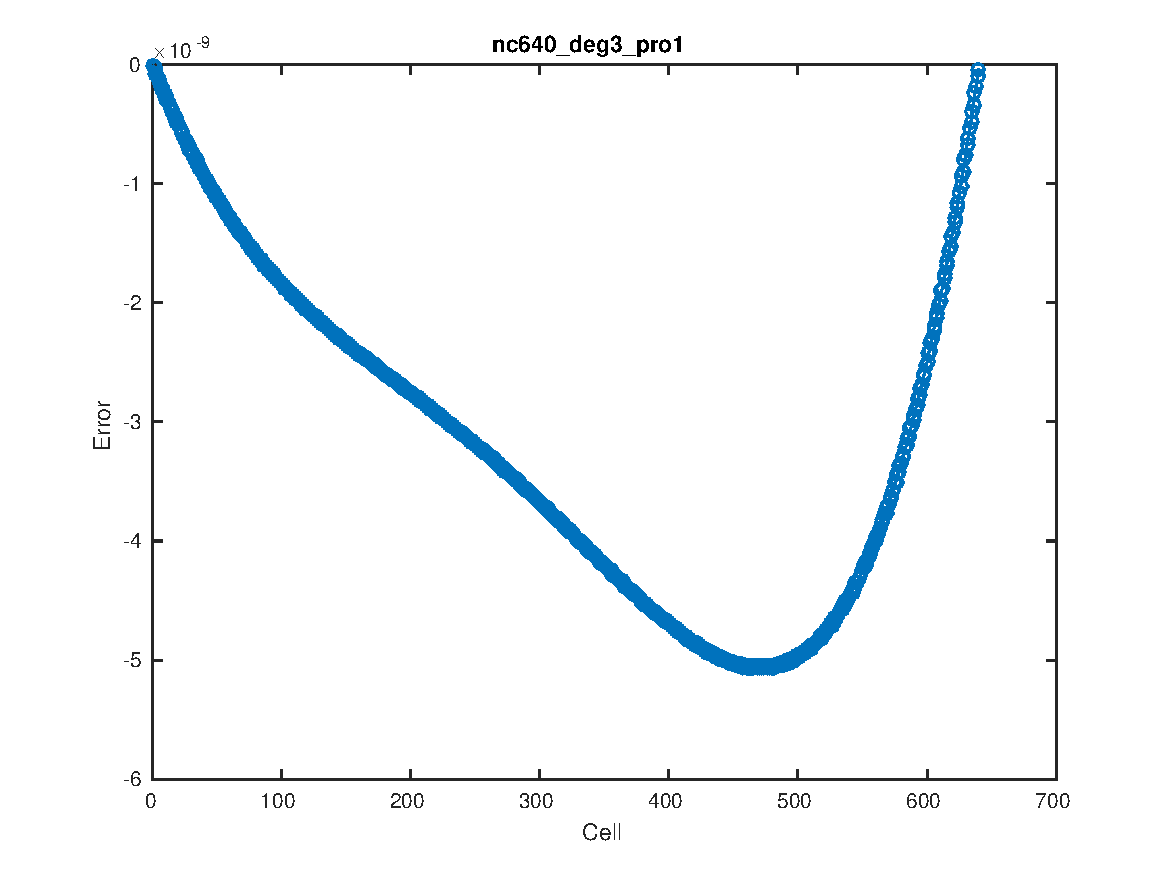
\includegraphics[width=\linewidth]{../../tests_01_01/test_01_01_test49_pro1/output/plots/nc640_deg3_wei111_pro1.pdf}
\end{subfigure}

\caption{$\omega=1|1,1$, d=3}
\end{figure}
%%%% 2
\begin{figure}[H]
\begin{subfigure}[b]{0.48\textwidth}
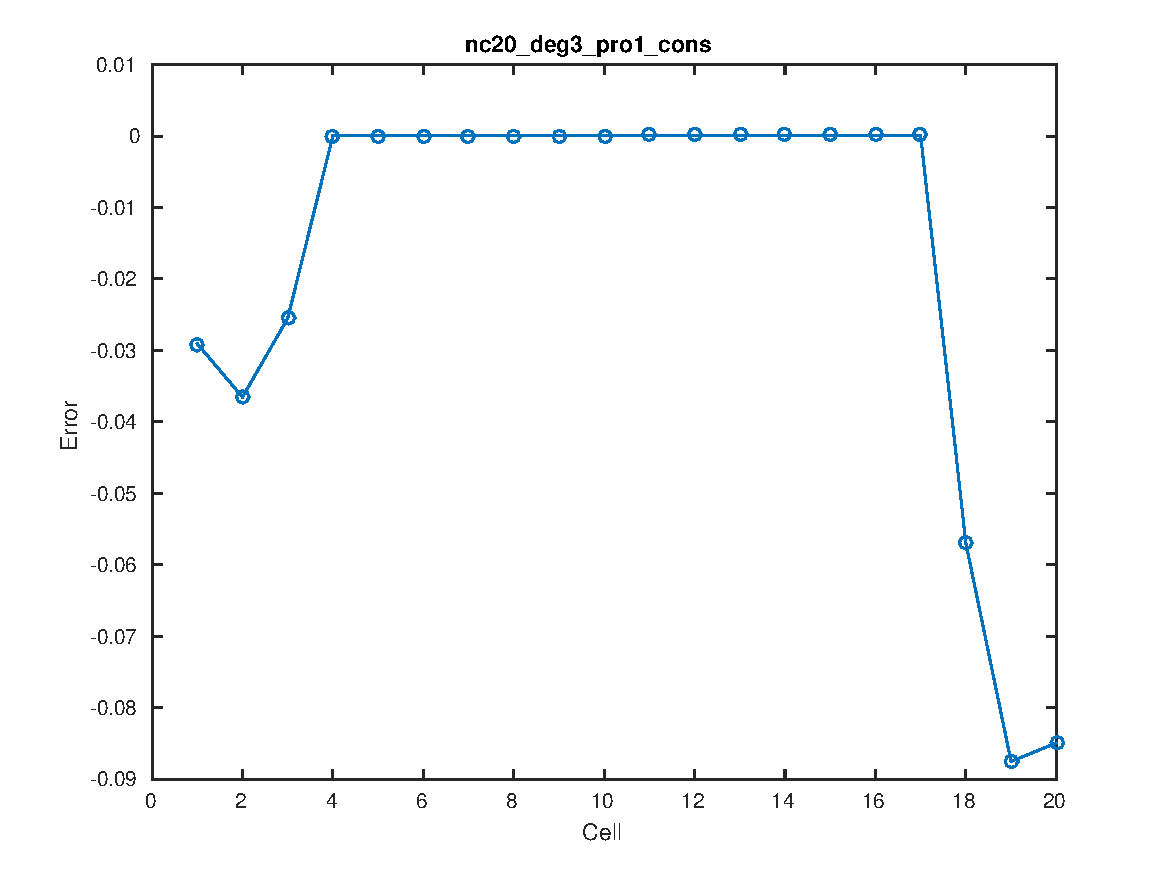
\includegraphics[width=\linewidth]{../../tests_01_01/test_01_01_test49_pro1_cons/output/plots/nc20_deg3_wei111_pro1_cons.pdf}
\end{subfigure}\hspace*{\fill}
\begin{subfigure}[b]{0.48\textwidth}
\includegraphics[width=\linewidth]{../../tests_01_01/test_01_01_test49_pro1_cons/output/plots/nc40_deg3_wei111_pro1_cons.pdf}
\end{subfigure}

\medskip
\begin{subfigure}[b]{0.48\textwidth}
\includegraphics[width=\linewidth]{../../tests_01_01/test_01_01_test49_pro1_cons/output/plots/nc80_deg3_wei111_pro1_cons.pdf}
\end{subfigure}\hspace*{\fill}
\begin{subfigure}[b]{0.48\textwidth}
\includegraphics[width=\linewidth]{../../tests_01_01/test_01_01_test49_pro1_cons/output/plots/nc160_deg3_wei111_pro1_cons.pdf}
\end{subfigure}

\medskip
\begin{subfigure}[b]{0.48\textwidth}
\includegraphics[width=\linewidth]{../../tests_01_01/test_01_01_test49_pro1_cons/output/plots/nc320_deg3_wei111_pro1_cons.pdf}
\end{subfigure}\hspace*{\fill}
\begin{subfigure}[b]{0.48\textwidth}
\includegraphics[width=\linewidth]{../../tests_01_01/test_01_01_test49_pro1_cons/output/plots/nc640_deg3_wei111_pro1_cons.pdf}
\end{subfigure}

\caption{$\omega=1|1,1$, d=3 (consistency)}
\end{figure}

\begin{figure}[H]
\centering
\includegraphics[width=.8\textwidth]{../../tests_01_01/test_01_01_test49_pro1_cons/output/plots/mesh.pdf}
\end{figure}
\pagebreak

\end{document}
% end of file